\documentclass{report}
\usepackage{graphicx} % Per le immagini
\usepackage{amsmath}
\usepackage{tikz} %grafi
\usepackage[hidelinks]{hyperref}% Collegamenti ipertestuali
\usepackage{verbatim}


\title{Interazione Multimedia}
\author{Damiano Trovato}
\date{2024/25}

\begin{document}


\maketitle
\renewcommand{\contentsname}{Indice}
\renewcommand{\chaptername}{Capitolo}
\newpage
\tableofcontents
\newpage
\chapter{Elaborazione delle Immagini (Prima lezione)}
È nella natura dell'uomo usare le immagini come mezzo di comunicazione.
È tra le forme più immediate ed efficaci.
Tuttavia, digitalizzare un'immagine richiede molto più spazio rispetto a delle stringhe di parole.\\
\textit{"Un'immagine vale più di mille parole... Solo che occupa più spazio!".}
\section{Cos'è un'immagine}
Generalmente, diciamo che un'immagine è una rappresentazione in due dimensioni di una realtà fisica, fotorealistica o immaginaria.
\section{Immagini e fotografia}
Il concetto di immagine viene associato spesso al concetto di fotografia.
Il primo documento fotografico risale al 1827, ed è di Joseph Nicéphore Niépce.
Data una lastra eliografica, e quindi di materiale fotosensibile, è possibile imprimere un'immagine su di essa.\\
La prima trasmissione di un'immagine risale al 1920.

\section{Elaborazione di un'Immagine Digitale}
La prima elaborazione digitale di un immagine, risale al 1964: è stata effettuata la correzione di alcune distorsioni ottiche di una foto della Luna, tramite un computer della NASA.
Elaborare un'immagine permette di facilitare la percezione di informazioni relative ad essa, come nel caso delle immagini satellitari, delle immagini ottenute dai raggi X nel campo medico e delle immagini a scopo forense.
Elaborare un'immagine significa applicare degli algoritmi di elaborazione.

\chapter{L'essere umano e le immagini}
Nell'essere umano, la percezione di un'immagine e la sua elaborazione sono compiti effettuati da parti diverse dell'organismo:
\begin{itemize}
	\item L'immagine viene impressa sulla retina, reagendo agli stimoli visivi
	\item Il cervello elabora l'immagine e associa ad essa un significato.
\end{itemize}
Mentre un'immagine è oggettiva, la percezione è spesso soggettiva, a causa della differente sensibilità alle intensità di colore e alle differenze cromatiche in soggetti diversi. 
\newpage
\section{Leggi della percezione visiva}
Nonostante la percezione visiva sia differente da individuo a individuo, esistono delle leggi che descrivono il modo di percepire insiemi di elementi, dette "leggi della percezione visiva".
\begin{itemize}
	\item \textbf{Legge della vicinanza}\\
	      Insiemi di elementi vicini tende ad essere percepito come unici.
	\item \textbf{Legge della chiusura}\\
	      La percezione delle figure chiuse prevale su quella delle figure aperte.
	\item \textbf{Legge dell'uguaglianza (o somiglianza):}\\
	      Elementi uguali che si assomigliano vengono percepiti come un insieme.
	\item \textbf{Legge della continuità}\\
	      Un insieme di punti consecutivi, e quindi posti l'uno di seguito all'altro, vengono percepiti come una struttura unica.
	\item \textbf{Legge delle buone forme}\\
	      La mente tende a vedere figure chiuse e completare figure incomplete, percependo forme regolari, strutture unitare e compatte.
	\item \textbf{Leggi della continuità}\\
	      La percezione delle linee come contorni degli oggetti, permettendoci di completare oggetti parzialmente coperti. Ci permette di percepire la tridimensionalità delle scene.
\end{itemize}

Molte di queste leggi sono alla base degli algoritmi di inpainting, capaci di eliminare elementi da foto e ricostruire la scena basandosi sugli elementi circostanti.
\begin{figure}[htp]
	\centering
	\includegraphics[width=10cm]{pic1.png}
	\caption{Esempi di Inpainting}
\end{figure}
\newpage
\section{Bande di Mach}
A sostegno della tesi per cui la percezione visiva è oggettiva e differente \\dall'intensità luminosa effettiva, portiamo come esempio le bande di Mach:\\
sono 5 bande grigie di 5 intensità diverse. Apparentemente l'intensità luminosa non è uniforme, e tende a cambiare in prossimità dei bordi delle bande, cosa che tuttavia, non avviene effettivamente.
Questo dimostra quindi che l'intensità luminosa viene percepita in maniera differente in ambienti scuri e in ambienti chiari.\\
È stato inoltre scientificamente dimostrato che l'intensità luminosa percepita cresce in maniera logaritmica rispetto a quella effettiva.
\begin{figure}[htp]
	\centering
	\includegraphics[width=8cm]{bandeDiMach.jpg}
	\caption{Bande di Mach: intensità effettiva vs percepita}
\end{figure}
\newpage
\chapter{Rappresentazione di un'immagine}
\section{Illuminazione e riflettanza}
Un'immagine è rappresentata da una funzione bidimensionale $f(x,y)$, dove $x$ e $y$ sono coordinate spaziali, e la $f(x, y)$ è proporzionale alla luce incidente nell'oggetto e riflessa da esso, e quindi:
$$f(x,y) = r(x,y) * i(x,y)$$
$$0 < i(x, y) < +\infty $$
$$ 0 < r(x,y) < 1 $$
Dove $i$ indica l'illuminazione ed $r$ la riflettanza.\\L'indice di riflettanza è relativo al materiale, ed è un numero limitato e compreso tra 0 e 1, a differenza dell'illuminazione, potenzialmente illimitato.
\section{Discretizzare per digitalizzare}
$f(x,y)$ è un valore reale dato dal prodotto descritto dalla formula precedente. Tuttavia, non potendo lavorare con valori reali, è fondamentale discretizzarli, e lo stesso vale anche per le variabili.\\
Le varibili $x$ e $y$ sono dette variabili spaziali o coordinate spaziali, appartengono al piano $XY$, per cui $f(x,y)$ indica l'intensità luminosa in un punto di coordinate $(x,y)$.

\section{Immagini vettoriali e Raster}
Le immagini Raster hanno un numero limitato di punti, dato dalla risoluzione dell'immagine.\\
L'idea dietro le immagini vettoriali, invece, è quella di descrivere le forme da creare come una lista di primitive geometriche.\\
Il programma si occuperà poi del rendering della grafica vettoriale, specificando il livello di dettaglio tramite la variabile Q di vettorializzazione.
La differenza tra Raster e vettoriale è chiara, in quanto le prime sono invece una collezione di pixel (abbreviazione di picture elements).\\
Date queste differenze, i due tipi di immagini si prestano a circostanze di tipo differente:
\begin{itemize}
	\item \textbf{Raster:}\\
	      Fotorealismo, disegno libero, immagini dettagliate e poco geometriche.
	\item \textbf{Vettoriale:}\\
	      Disegno geometrico, loghi, GIS, PDF, immagini e disegni da dettagli minimi.
\end{itemize}
\begin{figure}[htp]
	\centering
	\includegraphics[width=10cm]{vectorvsraster.jpg}
	\caption{Differenza tra immagine Vettoriale e Raster}
\end{figure}
Da ora in poi parleremo esclusivamente di immagini Raster.
\section{Immagini Raster come matrice}
Un'immagine Raster è una matrice di valori. Ciascuno di questi valori è associato all'intensità luminosa. Ciò significa che l'immagine è data dal variare dell'intensità luminosa $f(x,y)$ in ogni punto di coordinare $(x, y)$.\\
Per convenzione, poniamo sempre l'origine della matrice (o griglia) in alto a sinistra. Le coordinate sono sempre espresse in termini positivi.
\section{Tipologie di immagini}
\begin{itemize}
	\item \textbf{Bianco e nero:}\\
	      A ogni $(i, j)$ della matrice coincide un valore $f(i, j)$ variabile tra 0 e 1. Un singolo bit per punto. 0 coincide col nero, 1 coincide col bianco.
	\item \textbf{Scala di Grigi:}\\
	      A ogni $(i, j)$ della matrice coincide un valore $f(i, j)$ incluso tra 0 e 255. Vengono utilizzati 8 bit. 0 coincide col nero, 255 coincide col bianco.
	\item \textbf{A colori:}\\
	      Nel caso delle codifiche simil-RGB, ogni $(i, j)$ della matrice coincide un valore una terna di valori $f(i, j) = (x, y, z)$ inclusi tra 0 e 255. Vengono utilizzati 8 bit per canale, con 3 canali sono 24 bit in totale. 0 coincide con l'intensità minima della componente, 255 coincide con quella massima.\\
	      In codifiche alternative, i valori possono descrivere altre caratteristiche del colore di coordinate $(i, j)$. Ad esempio, con la codifica HSL indicheremo \textit{Hue, Saturation and Lightness}, ovvero crominanza, saturazione e luminosità.
\end{itemize}
\section{Immagini RGB}
Le immagini con codifica RGB sono risultato dell'unione di 3 canali (ciascuno per ogni componente di un colore) per punto: un canale dedicato alla componente rossa, uno a quella verde e uno a quella blu.
\newpage
\chapter{Operazioni su Immagini e Matrici}
Poter codificare un'immagine come una matrice, implica il poter operare\\
sull'immagine con le stesse operazioni definite per le matrici.\\
Tuttavia, non tutte le operazioni tra matrici sono sensate nell'ambito delle immagini. L'esempio più banale è il prodotto riga per colonna, che nella maggior parte dei casi, porta come risultato un'immagine irriconoscibile.
\section{Qualche nozione}
Il vicinato $N_p$ di un dato pixel sono i $p$ pixel adiacenti.\\
Esistono due tipi di vicinato p-connesso:
\begin{itemize}
	\item Vicinato 4 connesso include i 4 pixel adiacenti (sopra, sotto, sinistra e destra)
	\item Vicinato 8 connesso include anche i 4 pixel in diagonale.
\end{itemize}
\section{Trasformazioni affini}
Una trasformazione di rimappaggio delle coordinate prende in input delle coordinate, tornando in output delle nuove coordinate.\\ La trasformazione si dice affine se preserva tutti i parallelismi dell'immagine. Ogni trasformazione ha come risultato la modifica della posizione dei pixel dell'immagine.\\
Breve lista di operazioni affini:
\begin{itemize}
	\item \textbf{Identità:}\\
	      Non modifica l'immagine (la matrice).\\
	      T = Matrice identità.
	\item \textbf{Scaling:}\\
	      Altera le dimensioni sull'asse x e sull'asse y.
	      $
	      T =
	      \begin{bmatrix}
	      	c_x & 0   & 0 \\
	      	0   & c_y & 0 \\
	      	0   & 0   & 1 
	      \end{bmatrix}$
	\item \textbf{Rotazione:}\\
	      Ruota i pixel dell'immagine.
	      $
	      T =
	      \begin{bmatrix}
	      	cos\Theta  & sin\Theta & 0 \\
	      	-sin\Theta & cos\Theta & 0 \\
	      	0          & 0         & 1 
	      \end{bmatrix}
	      $
	\item \textbf{Traslazione:}\\
	      Sposta i pixel sui due assi.
	      $
	      T =
	      \begin{bmatrix}
	      	1   & 0   & 0 \\
	      	0   & 1   & 0 \\
	      	t_x & t_y & 1 
	      \end{bmatrix}
	      $
	\item \textbf{Shear verticale:}
	      $
	      T =
	      \begin{bmatrix}
	      	1   & 0 & 0 \\
	      	s_v & 1 & 0 \\
	      	0   & 0 & 1 
	      \end{bmatrix}
	      $
	\item \textbf{Shear orizzontale:}
	      $
	      T =
	      \begin{bmatrix}
	      	1 & s_h & 0 \\
	      	0 & 1   & 0 \\
	      	0 & 0   & 1 
	      \end{bmatrix}
	      $
\end{itemize}
Ogni trasformazione è quindi ottenuta moltiplicando la riga delle coordinate $[x, y, 1]$ (in coordinate omogeene) per la matrice di trasformazione $T$.

\section{Forward e backward (o inverse) mapping}
Nell'ambito dell'image processing, forward e backward mapping sono due approcci differenti alla trasformazione delle immagini (tramite funzione di rimappaggio).
\begin{itemize}
	\item \textbf{Forward mapping:}\\
	      Si scorre ogni pixel dell'immagine di input, si applica la matrice $T$ per calcolare la nuova posizione dei pixel nell'immagine d'output.
	\item \textbf{Backward mapping:}\\
	      Si scorre ogni pixel dell'immagine di output, campionando il pixel corretto dall'immagine di input, basandosi sulla matrice $T^{-1}$.
\end{itemize}

\subsection{Esempio di Backward mapping}
\textbf{Rotazione:}
$\Theta = \frac{\pi}{2}$
$$
T =
\begin{bmatrix}
	cos\Theta  & sin\Theta & 0 \\
	-sin\Theta & cos\Theta & 0 \\
	0          & 0         & 1 
\end{bmatrix};
$$
$$
T^{-1} =
\begin{bmatrix}
	cos\Theta & -sin\Theta & 0 \\
	sin\Theta & cos\Theta  & 0 \\
	0         & 0          & 1 
\end{bmatrix}
\Rightarrow 
\begin{bmatrix}
	0 & -1 & 0 \\
	1 & 0  & 0 \\
	0 & 0  & 1 
\end{bmatrix}
$$
È solo un caso che $T^{-1}$ sia la trasposta di $T$
Calcoliamo la posizione di alcuni pixel della seguente immagine (che rappresenteremo come matrice):
$
\begin{bmatrix}
	1 & 2 & 3 \\
	4 & 5 & 6 \\
	7 & 8 & 9 
\end{bmatrix}
$
$$
\textit{Coordinate di 1: } [0,0,1]
$$
$$
\textit{Coordinate di 2: } [0,1,1]
$$
$$
\textit{Coordinate di 3: } [0,2,1]
$$
\textit{Non scrivo le coordinate degli altri punti in quanto so già che finiranno fuori dall'immagine.}
$$
1: [0, 0, 1] * \begin{bmatrix}
0 & -1 & 0 \\
1 & 0 & 0 \\
0 & 0 & 1 
\end{bmatrix} = [0, 0, 1]
$$

$$
2: [1, 0, 1] * \begin{bmatrix}
0 & -1 & 0 \\
1 & 0 & 0 \\
0 & 0 & 1 
\end{bmatrix} = [0, -1, 1]
$$

$$
3: [2, 0, 1] * \begin{bmatrix}
0 & -1 & 0 \\
1 & 0 & 0 \\
0 & 0 & 1 
\end{bmatrix} = [0, -2, 1]
$$
\textit{Procederò calcolando la posizione degli altri pixel. Non scrivo i calcoli in quanto saranno tutti fuori dall'immagine di partenza.}\\
Immagine risultante:
$$
\begin{bmatrix}
	1 & X & X \\
	2 & X & X \\
	3 & X & X 
\end{bmatrix}
$$
Uso $X$ per indicare sezioni vuote.

\subsection{Vantaggi del Backward mapping}
Approcciandosi alla trasformazione a partire dall'immagine d'output, i calcoli saranno solo relativi ai pixel dell'immagine che vogliamo ottenere. Non andremo a calcolare la posizione di pixel out-of-bounds. \\ Risolviamo inoltre il problema dei buchi che possono essere generati con le trasformazioni in forward mapping, come nel caso dello scaling o della rotazione.
    
\newpage
\chapter{L'interpolazione}
È un'operazione matematica che ci permette di costruire la funzione interpolante $V(x,y)$, che permette di calcolare i valori non noti all'interno di uno o più intervalli cui estremi sono noti.

\section{Zooming in}
La trasformazione di scaling, nel caso specifico dello zooming in, genera \\un'immagine di dimensione maggiore da quella di partenza, con dei vuoti tra i pixel dell'immagine di partenza.\\
I seguenti algoritmi permettono di stimare in maniera più o meno adatta\\ l'intensità dei nuovi pixel intermedi.

\subsection{Nearest neighbour}
Sceglie il valore di intensità del pixel noto più vicino. A parità di vicinanza, segue una regola arbitraria. Algoritmo più semplice, scarsi risultati.
$$
\begin{bmatrix}
	10 & ? & 20 & ? \\
	?  & ? & ?  & ? \\
	30 & ? & 40 & ? \\
	?  & ? & ?  & ? \\
\end{bmatrix}
$$
Risultato:
$$
\begin{bmatrix}
	10 & 10 & 20 & 20 \\
	10 & 10 & 20 & 20 \\
	30 & 30 & 40 & 40 \\
	30 & 30 & 40 & 40 \\
\end{bmatrix}
$$
\subsection{Interpolazione bilineare}
Si prendono come riferimento i 4 pixel adiacenti (o più vicini) noti, per stimare l'intensità del pixel di intensità non nota.
Il valore assegnato si ottiene con l'equazione $V(x,y) = ax + by + cxy +d$\\
Esempio:
$$
\begin{bmatrix}
	10 & ? & 20 \\
	?  & ? & ?  \\
	30 & ? & 40 
\end{bmatrix}
$$
$$
\begin{cases}
	V(0,0): 10 = 0 + 0 + 0 + d   \\
	V(2,0): 20 = 2a + 0 + 0 + d  \\
	V(0,2): 30 = 0 + 2b + 0 + d  \\
	V(2,2): 40 = 2a + 2b + 0 + d 
\end{cases};
$$

$$
\begin{cases}
	V(0,0): d = 10           \\
	V(2,0): 2a + d = 20      \\
	V(0,2): 2b + d = 30      \\
	V(2,2): 2a + 2b + d = 40 
\end{cases};
$$

$$
\begin{cases}
	V(0,0): d = 10 \\
	V(2,0): a = 5  \\
	V(0,2): b = 10 \\
	V(2,2): c = 0  
\end{cases};
$$
Otteniamo la funzione:
$$
V(x,y) = 5x + 10y + 0xy + 10
$$
Calcolo il pixel di coordinate $(0, 1)$:
$$
V(0,1) = 10 + 10 = 20 
$$
Calcolo il pixel di coordinate $(1, 0)$:
$$
V(1,0) = 5 + 10 = 15
$$
Calcolo il pixel di coordinate $(1, 1)$:
$$
V(1,1) = 5 + 10 + 10 = 25 
$$
Calcolo il pixel di coordinate $(2, 1)$:
$$
V(2,1) = 10 + 10 + 10 = 30 
$$
Calcolo il pixel di coordinate $(1, 2)$:
$$
V(1,1) = 5 + 20 + 10 = 35 
$$

Immagine finale:
$$
\begin{bmatrix}
	10 & 15 & 20 \\
	20 & 25 & 30 \\
	30 & 35 & 40 
\end{bmatrix}
$$

\subsection{Interpolazione bicubica}
Utilizza i sedici pixel più vicini al punto.
$$
v(x,y) = \sum_{i=0}^{3} \sum_{j=0}^{3} a_{i,j} x^iy^j
$$
Non la approfondiamo, ma sappiamo che produce una formula di interpolazione molto accurata, grazie ai numerosi valori presi in considerazione per le stime. Più pesante computazionalmente.

\subsection{Problema dei bordi}
A ridosso dei bordi dell'immagine, il numero di pixel adiacenti è minore, e non risulterà possibile usare in maniera precisa gli algoritmi di interpolazione.
Due sono le possibili soluzioni:
\begin{itemize}
	\item Non fare nulla, replicando i valori di righe e colonne adiacenti.
	\item Usare un algoritmo che prende come riferimento un numero minore di pixel adiacenti.
\end{itemize}



\section{Zooming out}
Esistono anche dei metodi da usare nel caso dello zooming out, che genera immagini di dimensioni minori.
Esempio di soluzioni sulla seguente matrice:
$$
\begin{bmatrix}
	1  & 2  & 3  & 4  \\
	5  & 6  & 7  & 8  \\
	9  & 10 & 11 & 12 \\
	13 & 14 & 15 & 16 \\
\end{bmatrix}
$$

\subsection{Decimazione}
Teniamo un pixel seguendo una regola arbitraria (quello in alto a sinistra ogni 4 pixel, in questo caso):
$$
\begin{bmatrix}
	1 & 3  \\
	9 & 11 \\
\end{bmatrix}
$$

\subsection{Media}
In questo caso ogni due pixel in orizzontale e due in verticale, arrotondando per difetto:
$$
\begin{bmatrix}
	3  & 5  \\
	11 & 13 \\
\end{bmatrix}
$$
Procedure di calcolo della media hanno però un difetto, come vedremo spesso nel corso: possono generare nuovi colori inesistenti nell'immagine di partenza.
\newpage
\chapter{Stima della qualità di un algoritmo}
\section{MSE - Mean Square Error}
È un parametro usato per stimare l'errore quadrato medio tra due immagini, ed è direttamente proporzionale alle loro differenze.

\section{PSNR - Peak Signal to Noise Ratio}
Usato per valutare la qualità della compressione di un'immagine rispetto \\all'originale.
È una tecnica Full reference, ovvero richiede la presenza di due immagini, una di riferimento e una da valutare, e indicheremo la prima con $I(M \times N)$ e la seconda con $I'(M \times N)$.\\
Non è il miglior parametro per valutare un algoritmo di interpolazione, ma è il più diffuso.

\section{PSNR: Formule}
Calcolo del Mean Square Error (servirà per calcolare il PSNR)
$$ 
MSE = \frac{1}{MN}\sum^M_{x=1}\sum^N_{y=1} [ I'(x,y) - I(x,y)]^2
$$
PSNR - Varie formule equivalenti
$$
PSNR = -10log_{10}\frac{MSE}{S^2}
$$
$$
PSNR = 20log_{10}\frac{S}{\sqrt{MSE}}
$$
$$
PSNR = 10log_{10}\frac{S^2}{MSE}
$$
Dove $S$ è il valore massimo di intensità dei pixel (solitamente 255).
\subsection{Esempi di calcolo MSE e PSNR}
$$
G =
\begin{bmatrix}
	0 & 0 \\
	0 & 0 
\end{bmatrix}
$$
$$
G' =
\begin{bmatrix}
	255 & 255 \\
	255 & 255 
\end{bmatrix}
$$
$$
MSE(G, G') = \frac{1}{2*2}\sum^2_{x=1}\sum^2_{y=1}[G' - G]^2 = 255^2
$$

$$
I =
\begin{bmatrix}
	100 & 200 \\
	10  & 30  
\end{bmatrix}
$$
$$
I' =
\begin{bmatrix}
	101 & 201 \\
	12  & 28  
\end{bmatrix}
$$
$$
MSE(I, I') = \frac{1}{2*2}\sum^2_{x=1}\sum^2_{y=1}[I' - I]^2 = \frac{7}{4};
$$
$$
PSNR(I, I') = 10log_{10}\frac{255^2}{\frac{7}{4}} = 45,7;
$$
%%PROCESSING%
Il risultato del calcolo del PSNR è espresso in decibel ($10log_{10}$).\\
MSE e PSNR sono valori molto sensibili alle trasformazioni affini: confrontare un'immagine con la versione traslata, ruotata o ridimensionata di se stessa, avrà un forte impatto su valori di MSE e PSNR, per quanto sia molto semplice, per un essere umano, riconoscere le due immagini come uguali.
$$
MSE \in [0, 255^2] 
$$
\textit{O in generale il massimo numero rappresentabile col numero di bit dedicato all'intensità, al quadrato}
$$
PSNR \in [0, +n.bit^2[
	$$
		
	\section{Svantaggi del PSNR}
	Il PSNR non è un metodo che rispecchia alla perfezione il criterio umano: infatti, come l'essere umano riconoscerà le somiglianze tra due immagini trasformate, il PSNR potrebbe associare un valore di qualità molto alto a un immagine con molti pixel simili all'originale, ma cui soggetti sono irriconoscibili.
		
	\newpage
	\chapter{Acquisizione delle immagini digitali}
	Quando la luce colpisce un oggetto, parte di essa viene assorbita, l'altra viene riflessa. La riflessione dell'oggetto da origine al colore percepito. Catturare tramite un sensore la luce riflessa ed elaborarla, permette la creazione di un'immagine digitale.
		
	\section{Il sensore}
	L'ausilio di un sensore è fondamentale per catturare un'immagine digitale:\\
	l'energia che colpisce il sensore viene trasformata in inpulso elettrico. Esso sarà poi convertito in digitale.
	In strumenti diversi vengono utilizzati sensori di tipo differente:
	\begin{itemize}
		\item \textbf{Singolo sensore, spostamento in linea}:\\
		      Usato negli scanner, il sensore viene spostato lungo la sorgente da digitalizzare
		\item \textbf{Sensori disposti in 2D}:\\
		      Sono disposti in una matrice, permettono di catturare più punti contemporeaneamente senza richiedere uno spostamento, la cattura di tutti i sensori è simultanea. I più comuni sono i CCD.
	\end{itemize}
	\subsection{CCD: Charged Coupled Device}
	Dispositivi che si caricano positivamente se compiti da fotoni. Il numero di celle per area di esposizione è misurato in MEGAPIXEL. Le celle del CCD non possono caricarsi oltre una certa soglia (sovra-saturazione).
		
	\subsection{Dettagli sul processo di cattura}
	Successivamente all'acquisizione delle cariche da parte della matrice delle celle, avviene la scansione di ciascuna colonna della matrice. Essa richiederà un numero $C$ di fasi, dove $C$ è il numero di colonne. Scannerizzata la prima colonna, la carica già acquisita verrà spostata in memoria per fare spazio alle successive, che si sposteranno nella colonna appena liberata.
		
	\subsection{Cattura di un'immagine a colori}
	Non è possibile creare un tipo di sensore capace di catturare specifici colori, ma, usando un consono sistema di filtri, è possibile catturare i valori delle singole componenti dei colori.
		
	\subsection{Color Filter Array}
	È il nome con cui indichiamo la dispozione dei filtri colorati sui sensori. Il più usato, è il Bayer Pattern.
		
	\subsection{Bayer Pattern}
	È lo schema più utilizzato, sfrutta un rapporto 1:2:1 per i canali RGB. I pixel verdi sono disposti sulla diagonale.
		
	\begin{figure}[htp]
		\centering
		\includegraphics[width=0.5\linewidth]{bayer.png}
	\end{figure}
	Il risultato di una cattura tramite il Bayer Pattern, è in formato RAW. Il colorplane Bayer deve essere poi interpolato, tramite software, per ottenere i colori effettivi.
		
	\subsection{Color Interpolation}
	È il processo che permette di passare dall'immagine RAW, cui Bayer pattern è ancora riconoscibile (false-color), all'immagine cui colori sono quelli effettivi (true-color).
		
	\begin{figure}[htp]
		\centering
		\includegraphics[width=0.5\linewidth]{colorinterp.png}
	\end{figure}
	Esistono numerosi algoritmi usati nell'ambito della color interpolation.
	La nearest-neighbour interpolation, l'interpolazione bilineare o la bicubica possono essere usate per ricostruire i pixel delle immagini RGB.
	Dato un qualsiasi pixel, sarà solitamente noto uno dei suoi 3 valori RGB. Gli altri possono essere ottenuti tramite interpolazione. In questo modo, otterremo una terna di valori che indica il true-color.
	\newpage
	\chapter{Risoluzione}
	\section{Definizione e unità di misura}
	La più piccola e indivisibile unità di un'immagine Raster è un pixel.\\
	La risoluzione offre una misura sul quantitativo di pixel dedicati alla rappresentazione di un'immagine.
	Si dice risoluzione il numero di pixel per unità di misura.\\
	È misurabile in pixel al centimetro o dots per inch (dpi), o essere espressa come il numero di pixel su tutta l'immagine (esempio: 16 MegaPixel).
	\section{Risoluzione: indice di qualità?}
	È improprio dire che la risoluzione è indice di qualità di un'immagine?\\
	Una risoluzione piuttosto alta permette di rappresentare punti molto piccoli e indistinguibili, permettendo a un'immagine di non risultare sgranata.
	Tuttavia, la qualità dell'immagine, in termini di risoluzione, è il risultato della risoluzione dello strumento di ripresa e di quello di resa (esempio: fotocamera e monitor)
	\subsection{Risoluzione apparecchiatura di ripresa}
	È data dal numero di sensori per unità lineare di misura.
	Uno scanner arriva oltre i 6000 dpi. La risoluzione delle fotocamere è invece spesso espressa in MEGAPIXEL.
		
	\subsection{Risoluzione apparecchiatura di resa}
	È data dal numero di punti per unità lineare di misura.
	Gli schermi hanno tipicamente 72 dpi.\\
	Stampanti oltre 3000 dpi.\\
	Risoluzione di stampe:
	\begin{itemize}
		\item Quotidiano: 75 dpi
		\item Riviste; 133 dpi
		\item Brochure 175 dpi
		\item Libri Fotografici 2400 dpi
	\end{itemize}
	La risoluzione di un'immagine offre un'indice di "densità" di pixel, o punti, rispetto ad un'unità di misura: una densità maggiore si presta alla rappresentazione di determinate geometrie o immagini con un certo livello di dettaglio.\\
	La massima resa di un'immagine è data da un'equivalenza tra la risoluzione dell'immagine e di quello di resa: qualsiasi altra circostanza implica interpolazione.
	\subsection{Rapporto}
	Il rapporto di un'immagine offre un'informazione riguardo le proporzioni di altezza e larghezza della risoluzione dell'immagine.\\
	\textit{[Nota bene: i dpi non sono in relazione con la risoluzione e il rapporto.]}
	\newpage
	\chapter{L'occhio}
	\section{La retina}
	È una membrana che ricopre la parte posteriore dell'occhio, ed è costituita da coni e bastoncelli fotorecettivi. Intercettando stimoli luminosi, producono stimoli elettrici.
		
	\subsection{I coni}
	Sono circa 6/7 milioni, e sono concentrati principalmente nella zona centrale della retina, la fovea (/fò·ve·a/).\\
	Sono fortemente sensibili al colore, e ad ogni cono è collegato un nervo ottico. I coni distinguono specifiche lunghezze d'onda.
	\subsection{I bastoncelli}
	Sono circa 75/150 milioni, distribuiti su tutta la retina.
	Reagiscono all'intensità luminosa e non alla lunghezza d'onda. Sono i responsabili della vista scotopica (visione dell'occhio normale quando l'illuminamento degli oggetti è debole). Gruppi di bastoncelli sono collegati a singoli nervi.
	\subsection{Altro da sapere sulla retina}
	La fovea è una regione di $1,5 mm \times 1,5 mm$.
	Nella fovea sono presenti 150.000 coni per $mm^2$, per un totale di 337.500.
	Un CCD può contenere lo stesso numero di recettori in non meno di $5mm \times 5mm$.
	\section{Pinhole, cristallino e messa a fuoco}
	Il modello Pinhole è un modello che permette di astrarre il problema della formazione dell'immagine dell'occhio:\\
	Si approssima l'occhio a una scatola scura, foriamo con uno spillo (pin hole) una parete della scatola e poniamo, nella parete interna opposta al foro, una pellicola fotosensibile (che simula la retina).
	\begin{figure}[htp]
		\centering
		\includegraphics[width=0.57\linewidth]{pinhole.jpeg}
		\caption{Modello Pinhole}
	\end{figure}
	Il foro della pupilla, non essendo veramente puntiforme, permette l'accesso a più proiezioni di luce dallo stesso punto: la proiezione sulla retina di un punto dovrebbe di conseguenza diventare quella di un cerchio. Tuttavia, grazie alla deviazione del cristallino, la proiezione viene corretta. Il cristallino, infatti, essendo flessibile, si adatta alle distanze che vogliamo mettere a fuoco. 
		
	\section{Sulle fotocamere}
	Le lenti delle fotocamere non sono deformabili: per questo motivo, tramite un sistema manuale o automatico, è possibile cambiare la distanza della superficie fotosensibile rispetto al foro, per permettere la messa a fuoco di soggetti a varie distanze.
	Nel modello pinhole, il raggio del foro è proporzionale alla radice quadrata della distanza per la lunghezza d'onda della luce emessa.
	$$
	r = \sqrt{\lambda d}
	$$
	Tuttavia, per quanto un modello ideale del pinhole risulterebbe funzionante, un modello reale soffre di molti problemi:
	\begin{itemize}
		\item Il pinhole reale non presenta un foro puntiforme infinitesimo, in quanto non permetterebbe il passaggio della luce
		\item Il pinhole reale non può avere nemmeno un foro di dimensioni troppo piccole, in quanto genererebbe fenomeni di diffrazione.
		\item Un pinhole reale e funzionale presenta un foro di dimensioni notevoli ed una specifica forma geometrica. Per quanto questa "implementazione" sia funzionante, è soggetta a fenomeni di sovrapposizione di più fonti di luce.
		      \begin{figure}[htp]
		      	\centering
		      	\includegraphics[width=0.75\linewidth]{sovrapposizione.png}
		      	\caption{Sovrapposizione di due fonti luminose puntiformi}
		      \end{figure}
	\end{itemize}
		
	\section{Lenti sottili}
	I fori sono fondamentalmente inadeguati a tale compito: non permettono di recepire in maniera accurata spettri significativi di radiazione luminosa.
	Tuttavia, un risultato migliore può essere ottenuto con l'ausilio di lenti sottili, ovvero lenti dallo spessore trascurabile.
	\subsection{Proprietà geometriche della lente sottile}
	\begin{itemize}
		\item Raggi paralleli all'asse della lente sottile che passano attraverso essa, vengono proiettati tutti attraverso un punto specifico oltre la lente, chiamato fuoco.
		\item Una lente sottile ha due fuochi equidistanti da essa.
		\item Raggi che passano attraverso il fuoco, sono ritrasmetti tutti paralleli nella direzione dell'asse della lente.
	\end{itemize}
	\subsection{Equazione della lente sottile}
	Andiamo a trovare un'equazione che metta in relazione i valori indicati nella seguente immagine:
	\begin{figure}[htp]
		\centering
		\includegraphics[width=0.75\linewidth]{lentesottile.png}
	\end{figure}\\
	Individuando dei triangoli simili, possiamo arrivare alla seguente conclusione:
	$$
	u:(h+k) = f : h
	$$
	Conseguentemente: 
	$$\frac{u \cdot h}{f} = (h+k)$$
	Analogamente, diremo anche che:
	$$
	v:(h+k) = f:k
	$$
	Conseguentemente:
	$$\frac{v \cdot k}{f} = (h+k)$$
	Eguagliamo:
	$$
	\frac{v \cdot k}{f} = \frac{u \cdot h}{f}
	$$
	$$
	\frac{h}{v} = \frac{k}{u}
	$$
	Da $(h+k) = \frac{u \cdot h}{f}$ dividiamo entrambi i membri per $u$ ottenendo:
	$$
	\frac{h}{u} + \frac{k}{v} = \frac{h}{f}
	$$
	Ma $\frac{k}{u} = \frac{h}{v}$, e quindi;
	$$
	\frac{h}{u} + \frac{h}{v} = \frac{h}{f}
	$$
	Eliminiamo il fattore comune e ottendiamo definitivamente l'equazione della lente sottile, ovvero:
	$$
	\frac{1}{u} + \frac{1}{v} = \frac{1}{f}
	$$
	\subsection{Messa a fuoco, equazione della lente sottile}
	Se $f$ si misura in metri, $\frac{1}{f} = 1$ diottria.
	\begin{itemize}
		\item Quando abbiamo una lente fissa, come nelle fotocamere, $f$ è una quantità costante. Se la distanza dall'oggetto indicata con $u$ aumenta, la distanza lente -  sensore deve diminuire., 
		\item Se il piano dei sensori non può allontanarsi, come nel caso della pupilla, e quindi $v$ è fissa, ciò che possiamo fare è aggiustare la lunghezza focale ($f$), mettendo in tensione il cristallino. 
		\item Due oggetti a distanza $u_1$ e $u_2$ dalla lente sottile, distanze di molto superiori a $f$, appariranno approssimatamente sullo stesso piano (in quanto $v_1$ e $v_2$ saranno valori molto vicini);
		      ciò non succede invece quando $u_1$ ed $u_2$ sono a distanze differenti e comparabili (meno di 30 volte la distanza della lente), allora non sono focalizzabili contemporaneamente. Si presenterà così il fenomeno della "profondità di campo".
	\end{itemize}
	\subsection{Magnificazione}
	Col termine magnificazione andiamo a indicare la proprietà, della lente sottile, di alterare la dimensione dell'immagine di un oggetto rispetto alla dimensione effettiva di esso.
	Il fattore di magnificazione è dato da: $$\frac{h}{k} = \frac{v}{u} = m$$
	Moltiplichiamo per $v$ l'equazione della lente sottile
	$$
	\frac{v}{u} + 1 = \frac{v}{f}
	$$
	Ovvero
	$$
	m + 1 = \frac{v}{f}
	$$
	Invertiamo:
	$$
	\frac{1}{m+1} = \frac{f}{v}
	$$
	Moltiplichiamo per $u$ e sostituiamo $\frac{u}{v} = \frac{1}{m}$.
	$$
	\frac{u}{m+1} = \frac{f}{m}
	$$
	Moltiplichiamo per $m$ ottenendo finalmente una relazione tra il fuoco, la distanza dall'oggetto e il fattore di magnificazione.
	$$
	f = u \cdot \frac{m}{m+1}
	$$
	\textit{[Annoto qua per comodità tutte le variabili:]}
	\begin{itemize}
		\item $u$ - distanza oggetto - lente
		\item $v$ - distanza lente - sensore
		\item $f$ - fuoco
		\item $m$ - fattore di magnificazione
	\end{itemize}
		
	\subsection{Esercizi sul calcolo:}
	\begin{itemize}
		\item 
		      		      
		      Oggetto a distanza $u=1cm$.\\
		      Macchina analogica con $v=2cm$.\\
		      Se la farfalla è a distanza $u_1=5cm$ si ha $m=\frac{2}{1}=2$ e $f=5 \cdot \frac{2}{3}=3.3cm$
	\end{itemize}
	\newpage
	\chapter{Campionamento e Quantizzazione}
	\section{In cosa consistono?}
	Per effettuarne una digitalizzazione di un segnale analogico e continuo, occorre scegliere un numero finito di "campioni" rappresentativi del segnale.\\
	Se nel segnale analogico il valore in ogni singolo punto è un numero reale, la controparte digitale sarà costituita da valori discreti opportunatamente scelti.
	Nella seguente immagine, abbiamo un esempio di campionamento e quantizzazione:
	\begin{figure}[htp]
		\centering
		\includegraphics[width=0.6\linewidth]{Basic-Concepts-in-Sampling-and-Quantization.jpeg}
	\end{figure}\\
	All'insieme continuo di valori di intensità dell'immagine, viene associato un insieme discreto di valori.
	\section{Campionamento}
	Consiste nell'acquisizione di campioni all'interno di un segnale analogico continuo. Il tasso di campionamento indica il numero di volte in cui avviene il campionamento del segnale in un determinato lasso di tempo.
	La scelta del tasso di campionamento è fondamentale:
	un campionamento \\troppo basso fa perdere dettagli o causare fenomeni di aliasing
	\subsection{Nyquist Rate}
	Si definisce Nyquist rate il doppio della più alta frequenza di un segnale continuo e limitato. Nel pratico, rappresenta il dettaglio più piccolo rappresentabile in un segnale.
	\subsection{Teorema di Shannon}
	Raccogliere un numero di campioni maggiore al Nyquist Rate ci permette di ricostruire il segnale fedelemente in ogni suo punto. Usiamo questo teorema per scegliere opportunamente la frequenza di campionamento.
	\subsection{Aliasing}
	Derivante dal termine "alias", si riferisce al mascheramento delle alte frequenze come basse frequenze nella fase di campionamento. Questo genera artefatti, "righette" orizzontali e verticali. Spariscono inotre dettagli o vengono generate distorsioni in prossimita di linee continue.
	\begin{figure}[htp]
		\centering
		\includegraphics[width=1\linewidth]{aliasingexample.png}
		\caption{Esempi di Aliasing}
	\end{figure}
	Un tipo di artefatto particolare generato da una frequenza di campionamento troppo bassa, è chiamato "Moiré pattern". Nella seguente immagine è visibile in prossimità dell'orizzonte.
	\begin{figure}[htp]
		\centering
		\includegraphics[width=0.7\linewidth]{moirepattern.png}
		\caption{Esempi di Aliasing, Moiré Pattern}
	\end{figure}
	\subsection{Undersampling e aliasing temporale}
	Nell'ambito dei video, un framerate basso potrebbe causare problemi relativi alla percezione del movimento degli oggetti, un vero e proprio alias temporale. Un movimento rotatorio in un verso, dato un basso framerate, potrebbe rendere in video nel verso opposto.
	\begin{figure}[htp]
		\centering
		\includegraphics[width=1\linewidth]{wheel.png}
	\end{figure}
	\section{Quantizzazione}
	È il processo di discretizzazione dei valori reali catturati dopo il campionamento. \\
	I sensori, essendo apparati fisici, possono catturare valori continui, ma anche subire interferenze.
		
	\subsection{Procedura generale di quantizzazione}
	I valori da quantizzare sono nel range $[a,b]$ e si vuole quantizzare su $n$ livelli:
	\begin{itemize}
		\item Si fissano $n+1$ numeri ($t_0,t_1,...t_n$) $\in [a,b]$ tali che:
		      $$
		      t_0 = a < t_1 < t_2 < ... < t_n = b
		      $$
		\item Il numero $x \in [a,b]$ verrà assegnato al livello di quantizzazione $k$ se risulta:
		      $$
		      t_k \leq x < t_{k+1}
		      $$
		      $b$ viene assegnato a $t_k$.
	\end{itemize}
	\subsection{Implicazioni della quantizzazione}
		
	Ogni segnale, quando viene quantizzato, presentirà di distorsioni di quantizzazione. È impossibile andare a quantizzare un segnale continuo senza introdurre un minimo di distorsione di quantizzazione, in quanto non è possibile ricostruire un segnale continuo in ogni suo punto, in quanto infiniti. Tuttavia, una quantizzazione su molti livelli permetterà di rendere il meno percettibile possibile la differenza tra il segnare analogico e quello digitalizzato.
		
	\subsection{Distribuzione dei livelli di quantizzazione}
	Quantizzare, significa associare e dei range di frequenze, dei valori discreti.\\
	Questi range possono essere di dimensione uniforme o non uniforme.
	\begin{itemize}
		\item \textbf{Uniforme:}\\
		      I range che vengono associati ad un valore sono di dimensione costante. Non richiede uno studio specifico.
		\item \textbf{Non Uniforme:}\\
		      I range che vengono associati ad un valore sono di dimensione non costante. Conoscendo la percezione umana dell'intensità luminosa, o del range di frequenze in generale, è possibile creare una quantizzazione ad hoc, con una resa migliore rispetto al contesto.
	\end{itemize}
		
	\subsection{Quantizzazione Uniforme}
	La quantizzazione avviene per mezzo di una funzione lineare
	$$
	L' = \frac{L \cdot K}{N}
	$$
	Dove:
	\begin{itemize}
		\item $L$ è il livello di ingresso rappresentato da un intero.
		\item $L'$ è il livello post-quantizzazione.
		\item $N$ è il numero di livelli del range in ingresso $(0, ..., N-1)$.
		\item $K$ è il numero di livelli del range in uscita $(0, ..., K-1)$.
	\end{itemize}
	\subsection{Esempio di quantizzazione uniforme}
	Immagine a 8 bit $\Rightarrow$ 256 livelli.\\
	$N = 256$
	$$
	M = 
	\begin{bmatrix}
		0  & 100 \\
		50 & 200 
	\end{bmatrix}
	$$
	Vogliamo quantizzarla a 3 bit $\Rightarrow$ 8 livelli.\\
	$K = 8$
	$$
	L'_{11} = (0 \cdot 8)/256 = 0
	$$
	$$
	L'_{12} = (100 \cdot 8)/256 = 3,125
	$$
	$$
	L'_{21} = (50 \cdot 8)/256 = 1,56
	$$
	$$
	L'_{22} = (200 \cdot 8)/256 = 6,25
	$$
	Prendiamo solo la parte intera dei numeri reali ottenuti. Matrice risultante:
	$$
	M' = 
	\begin{bmatrix}
		0 & 3 \\
		1 & 6 
	\end{bmatrix}
	$$
		
	\subsection{Quantizzazione non-uniforme}
	La quantizzazione non uniforme avviene per mezzo di una funzione nella forma
	$$
	L' = \frac{f(L) \cdot K}{f(N)}
	$$
	Dove:
	\begin{itemize}
		\item $L$ è il livello di ingresso rappresentato da un intero.
		\item $L'$ è il livello post-quantizzazione.
		\item $N$ è il numero di livelli del range in ingresso $(0, ..., N-1)$.
		\item $K$ è il numero di livelli del range in uscita $(0, ..., K-1)$.
		\item $f(n)$ è una funzione a scelta. La più tipica, è quella logaritmica $log_2(n)$, e quindi:
		      $$
		      L' = \frac{log_2(L) \cdot K}{log_2(N)}
		      $$
	\end{itemize}
		
		
		
	\subsection{Esempio di quantizzazione non-uniforme (logaritmica)}
	Immagine a 8 bit $\Rightarrow$ 256 livelli.\\
	$N = 256$
	$$
	M = 
	\begin{bmatrix}
		0  & 100 \\
		50 & 200 
	\end{bmatrix}
	$$
	Vogliamo quantizzarla a 3 bit $\Rightarrow$ 8 livelli.\\
	$K = 8$
	$$
	L'_{11} = (log_2(0) \cdot 8)/log_2(256) = \textit{Non calcolabile} = 0
	$$
	$$
	L'_{12} = (log_2(100) \cdot 8)/log_2(256) = log_2(100) = 6,64
	$$
	$$
	L'_{21} = (log_2(50) \cdot 8)/log_2(256) = log_2(50) =
	$$
	$$
	L'_{22} = (log_2(200) \cdot 8)/log_2(256) = log_2(200) =
	$$
	Prendiamo solo la parte intera dei numeri reali ottenuti. Matrice risultante:
	$$
	M' = 
	\begin{bmatrix}
		0 & 3 \\
		1 & 6 
	\end{bmatrix}
	$$
	\newpage
	\chapter{Colore}
	\section{I colori come onda elettromagnetica}
	Un raggio luminoso di colore bianco, attraverso un prisma di vetro, viene suddiviso nel suo spettro. Chiameremo questo spettro "luce visibile", ed include tutte quelle lunghezze donda tali da appartenere a questo spettro.
	\subsection{Lo spettro elettromagnetico}
	Le onde elettromagnetiche visibili appartengono ad un range, chiamato "range della luce visibile". Sono onde cui stimoli fanno reagire la retina.
	Le lunghezze d'onda del range visibile vanno da circa 400 nanometri a 700 nanometri. Subito sotto i 400 nanometri abbiamo gli infrarossi, oltre i 700 nanometri abbiamo gli ultravioletti.
	$$
	\lambda * f = c
	$$
	Dove $\lambda$ e $f$ sono rispettivamente lunghezza d'onda e frequenza delle onde elettromagnetiche. $c$ è la costante che indica la velocità della luce.
	\subsection{La luce visibile}
	Abbiamo già detto che la luce visibile è nel range dei $[400nm,700nm]$.
	Dividiamo per comodità lo spettro in sei regioni di dimensione irregolare: violetto, blu, verde, giallo, arancio e rosso.
	\subsection{Percezione del colore degli oggetti}
	L'essere umano percepisce il colore di un oggetto la componente di luce che non viene assorbita, e bensì riflessa dall'oggetto.\\
	Questo significa che un oggetto cui superficie assorbe tutte le regioni dello spettro della luce visibile, eccetto la regione verde, risulterà proprio di colore verde.
	\subsection{Descrivere la luce}
	Sono tre i valori sufficienti a descrivere la luce:
	\begin{itemize}
		\item Radianza: quantità di luce emessa dalla sorgente luminosa
		\item Luminanza: energia percepita dall'utente
		\item Brillantezza: un valore soggettivo che indica la sensazione di colore
	\end{itemize}
		
	\subsection{I coni e il loro spettro di assorbimento}
	Nella retina sono presenti tre tipi di coni.
	\begin{itemize}
		\item \textbf{Tipo S}\\
		      Lunghezze d'onda corte, short, colori bluastri
		\item \textbf{Tipo M}\\
		      Lunghezze d'onda medie, middle, verdastri
		\item \textbf{Tipo L}\\
		      Lunghezze d'onda lunghe, long, rossastri
	\end{itemize}
	\begin{figure}[htp]
		\centering
		\includegraphics[width=0.5\linewidth]{assorbimento.png}
	\end{figure}
	\section{Colore e soggettività:}
	Il riconoscimento dei colori da parte dell'uomo è basato sulla luce, sugli oggetti che riflettono la luce e sugli occhi e il cervello dell'osservatore.
	\subsection{Differenze di colore}
	Elementi che portano a differenze nelle percezioni di colore.
	\begin{itemize}
		\item \textbf{Differenze di sorgenti luminose:}\\
		      Luce nell'ambiente circostante.
		\item \textbf{Differenze di osservatore:} \\
		      Sensibilità differenti al colore
		\item \textbf{Differenze di dimensioni:} \\
		      Effetto area = colori che ricoprono spazi più vasti appaiono più vivaci e luminosi
		\item \textbf{Differenze di sfondo:} \\
		      Effetto contrasto = colori più cupi se lo sfondo è scuro
		\item \textbf{Differenze di direzione:} \\
		      Caratteristche direzionali di alcune vernici.
	\end{itemize}
		
	\chapter{Spazi di colore}
	\section{Introduzione agli spazi di colore}
	Gli spazi di colore nascono con lo scopo di permettere la specificazione di colori, con modalità standardizzate, che fanno solitamente riferimento ad un sistema di coordinate all'interno di un sottospazio tridimensionale, nel quale ogni colore è rappresentato da un punto.\\
	Introduciamo questo capitolo con la sfatata teoria del tristimolo.
	\subsection{Teoria del tristimolo (Young, 1802)}
	È l'ipotesi secondo cui ogni colore può essere ottenuto mescolando tre colori fondamentali in proporzioni differenti. Nonostante la sua incorrettezza, è stata alla base delle codifiche utilizzate ancora oggi per i colori.
		
	\subsection{Composizione dei colori}
	Illuminando una superficie bianca (coefficiente di riflessione del 100\%) con una o più luci monocromatiche, si ottiene (per riflessione) una radiazione colorata per sintesi additiva.\\
	Partendo dalla ipotesi che ogni colore possa essere valutato in termini di tre componenti pure, la CIE (Commissione Internazionale per l'Illuminazione) ha scelto le tre radiazioni primarie in modo che le lunghezze d'onda siano il più possibile distanziate nello spettro, ottenendo quindi:
	$$
	Blu = 435,8 \ nm; \ Verde = 546,1 \ nm; \ Rosso=700 \ nm
	$$
	Anche se dati sperimentali hanno dimostrato che il valore reale è lievemente differente:
	$$
	Blu = 445 \ nm; \ Verde = 535 \ nm; \ Rosso=575 \ nm
	$$
	\subsection{Colori primari e secondari}
	Chiameremo rosso, verde e blu "colori primari" o "primari additivi", e combinando i colori in questione due a due, otteniamo i "colori secondari", o "primari sottrattivi", ovvero magenta, ciano e giallo.
	\subsection{Diagramma cromatico CIE}
	\begin{itemize}
		\item $x$ è la quantità di rosso
		\item $y$ è la quantità di verde
		\item $z = 1-(x+y)$ è la quantità di blu
	\end{itemize}
	La rappresentazione grafica al variare di $x$ e $y$ da origine al diagramma cromatico CIE, di cui possiamo denotare alcune caratteristiche interessanti:
	\begin{itemize}
		\item Il punto di uguale energia tra le tre componenti contiene il bianco. Tutti i punti ai bordi non ha bianco, e sono detti colori puri.
		\item Unendo due colori con una linea, tutti i colori nella linea sono ottenibili mescolando i due colori
		\item Unendo un colore con il bianco si ottengono tutte le tonalità di quel colore.
		\item Unendo tre colori con un triangolo, tutti i colori lungo il bordo e nel triangolo sono quelli ottenibili mischiando quei tre colori
		\item Notiamo inoltre il triangolo di spigoli R, G, B non copre tutta l'area del diagramma cromatico, sfatando quindi la teoria del tristimolo.
	\end{itemize}
	Se permettiamo a questi tre valori di variare, diventa chiaramente possibile rappresentare ogni colore dello spettro visibile. Tuttavia, ciò implica l'impossibilà di fissare tre componenti fondamentali standard.
		
	\begin{figure}[htp]
		\centering
		\includegraphics[width=0.3\linewidth]{gamut.png}
		\caption{Color gamut (gamma di colori)}
	\end{figure}
	L'area convessa più grande include tutta la luce visibile. Il triangolo unisce le tre lunghezze d'onda fissate dallo standard CIE. L'area ulteriormente più piccola inscritta nel triangolo, è la gamma di colori di una stampante (colori ottenuti per sintesi sottrattiva)
	\newpage
	\subsection{Spazi percettivamente non uniformi}
	Un problema relativo agli spazi di colore del sistema CIE è quello legato alla non-uniformità:\\
	due colori equidistanti da due valori, non sono percepiti come equidistanti.
	\subsection{CIELAB}
	È, assieme allo spazio L*u*v*, uno spazio di colore percettivamente uniforme.
	$L*$ indica la luminanza, $a*$ e $b*$ la crominanza.
	Sono tutti e tre trasformazioni dei valori di tristimolo $X,Y,Z$ dello spazio di colore $CIE \ XYZ$.
	Nello spazio di colore in questione, le differenze di colore sono definite come distanze tra due punti:
	$$
	\Delta E^*_{ab} = \sqrt{\Delta L^{*2} + \Delta a L^{*2} + \Delta b L^{*2}}
	$$
	$L^* = 100$: bianco, $L^*=0$: nero, $a^*,b^* =$ coordinate di cromaticità.
		
	\subsection{Spazio LCh}
	Chroma:
	$$C^* = \sqrt{(a^*)^2 + (b^*)^2}$$
	Hue angle:
	$$h = \tan^{-1}(\frac{b^*}{a^*})$$
	\newpage
	\section{Spazio di colore HSV}
	\subsection{Illuminanti}
	Si definisce come illuminante una luce teorica, presumibilmente dalla\\distribuzione spettrale nota, capace di alterare il colore percepito degli oggetti. Lo spettro di un illuminante è il diagramma dei contributi di energia che esso apporta a ciascuna differente lunghezza d'onda.
	\subsubsection{I metameri}
	Due spettri diversi capaci di produrre medesimi colori, sono detti "metameri".
	\subsection{Modello del pittore}
	Ad ogni spettro di illuminante coincide un metamero nella seguente forma:\\
	\begin{figure}[htp]
		\centering
		\includegraphics[width=1\linewidth]{modellodelpittore.png}
	\end{figure}
	Chiameremo la lunghezza d'onda del picco "hue", in italiano "colore percepito". Il rapporto $\frac{e_{picco}- e_{media}}{e_{picco} + e_{media}}$ è detto "saturazione". La $e_{media}$ è proporzionale al contenuto energetico della radiazione, e da contributo bianco al colore percepito.
	Ad ogni colore percepito (hue) coincide un triangolo:\\
	\begin{figure}[htp]
		\centering
		\includegraphics[width=1\linewidth]{hue1.png}
	\end{figure}
	Unendo, geometricamente parlando, i triangoli, otterremo lo spazio di colore $HSV$, rappresentato, per l'appunto, da un cono.
	$\\ H = hue;\\ \ S = saturazione \ o \ C = chroma ;\\ \ V = valore;$
		
		
	\section{Spazi di colore RGB e CMY}
	\subsection{Sintesi additiva}
	La composizione additiva dei colori è il principio alla base del funzionamento dei monitor. I colori vengono creati a partire dai tre "colori primari" rosso, verde e blu. Inoltre, combinando a due a due i colori, otteniamo giallo, magenta e ciano. Dalla sovrapposizione di tutti e tre i colori, otteniamo il bianco. Viene replicata illuminando con tre fasci di luce colorati.
	\subsection{Sintesi sottrattiva}
	La sintesi sottrattiva, ottenuta sovrapponendo dei filtri ciano, giallo e magenta.
	$Y+M=R; \ Y + C = G; \ M + C = B; \ Y+M+C = K$
	\subsection{RGB}
	Nel modello RGB ogni colore viene ottenuto mischiando i tre colori fondamentali. Considerando ogni componente come una coordinata cartesiana, il modello RGB è descrivibile come un cubo. Il suo complementare è lo spazio di colore CMY.
	\subsection{}section{Colori sicuri per il web}
	Il web usa tipicamente 256 colori. Mentre 40 di questi sono processati diversamente da i vari sistemi operativi, gli altri 216 sono comuni alla maggior parte di loro, e sono detti web-safe colors.
	Il loro esadecimale ha la caratteristica di essere formato solo da i seguenti numeri: 00, 33, 66, 99, CC, FF.
	\section{Famiglia di spazi di colore YUV}
	In questo tipo di spazi di colore, utilizzato per la codifica di immagini o video analogici, i valori di luminanza e crominanza sono tenuti separati.\\
	Tra le controparti digitali degli spazi YUV, troviamo gli spazi $YC_bC_r$.
	\subsection{Da RGB a YUV}
	Nel caso in cui R, G e B siano compresi tra 0 e 1, si ottengono valori di Y compresi tra 0 e 1, e valori di U e V compresi tra -0,5 e 0,5.
	\subsection{Da RGB e YUV a YCbCr}
	$$
	Y = 0.299R + 0.587G + 0.114B \textbf{(presente nell'ultima prova in itinere!)}
	$$
	$$
	C_b = U + 128
	$$
	$$
	C_r = V + 128
	$$
	\newpage
	\chapter{Colori e Memoria}
	Memorizzare le informazioni relative ai colori dei pixel che compongono \\un'immagine, implicherebbe l'utilizzo di una matrice di dimensioni pari alla risoluzione, contenenti terne di 8 bit. \\
	Questo metodo tuttavia è spesso sconveniente, soprattutto per immagini a pochi colori. Andiamo quindi a introdurre delle alternative.
	\section{Immagini a colori indicizzati}
	Piuttosto che creare una matrice di terne, andremo a creare una tabella contenente terne assieme ad un indice univoco associato ad ogni colore.\\
	In questo modo, possiamo andare a memorizzare ogni pixel usando memoria pari $2^n$, con $n$ colori.
	La tabella in questione si chiama tavolozza o palette.
	\section{Re-indexing}
	Esistono strategie di compressione applicabili alle matrici degli indici delle immagini a colori indicizzati.\\
	Un'immagine a $n$ colori avrà $n$ indici differenti.
	Ogni immagine sarà quindi rappresentabile in $n!$ modi ($n!$ permutazioni), in quanto ad ogni terna potremmo associare uno tra gli $n$ indici disponibili.
	Scegliendo la permutazione ottimale, è possibile ottenere un'entropia più bassa nell'immagine, permettendo agli algoritmi di compressione di funzionare nella maniera migliore.
	Idealmente, la permutazione migliore associa a indirizzi simili, colori simili.
	\begin{figure}[htp]
		\centering
		\includegraphics[width=0.85\linewidth]{Immagine WhatsApp 2024-11-14 ore 09.11.45_0c410681.jpg}
	\end{figure}
	\newpage
	\chapter{Istogramma}
	Le immagini sono collezioni di valori numerici.
	Lavorando con lavori numerici, è possibile andare a tracciare istogrammi che permettono di rappresentare le occorrenze di un determinato valore all'interno dell'immagine.
	Un'istogramma è implementabile come un vettore di elementi.
	Un'istogramma è detto normalizzato quando ogni elemento del vettore è espresso come $\frac{occorrenze}{occorrenze \; totali}$
	\section{Caratteristiche dell'immagini}
	Un'istogramma ordinato permette di capire la distribuzione delle occorrenze di determinati toni di grigio.
	L'istogramma di un'immagine che subisce trasformazioni legate all'ordine dei pixel, rimane costante.\\
	Istogramma diverso $\Rightarrow$ Immagine diversa.\\
	Tramite gli istogrammi, ad esempio, è possibile intuire se un'immagine è sovraesposta o sottoesposta.
	\section{Contrast Stretching}
	È un'operazione che, operando sull'istogramma, permette di ottenere una distribuzione sull'istogramma che copre l'intero range dei colori.
	\subsection{Formula di Normalizzazione Lineare}
	Di seguito, la formula usata dall'operazione di contrast stretching. [N.B. non c'entra nulla con la definizione di istogramma normalizzato]
	$$
	v_{nuovo} = 255 \cdot \frac{(v_{vecchio} - min_{osservato})}{(max_{osservato} - min_{osservato})}
	$$
	Che ritorna il valore di $v$ nel nuovo range $[0,255]$.
	\subsection{Contrast stretching su immagini a colori}
	Ogni immagine a colori avrà tre istogrammi.
	Effettuare un'operazione di contrast stretching su un'immagine cui colori non hanno una distribuzione uniforme e range dinamici tra colori differenti, potrebbe farci ottenere un'immagine dai colori più naturali.
	\section{Equalizzazione}
	È un'operazione che attenua le differenze tra occorrenze\\ dei pixel di valore diverso. Tende, in un certo senso, ad appiattire l'istogramma relativo all'immagine.
	\subsection{Algoritmo di Equalizzazione}
	Definiamo prima l'istogramma normalizzato:\\
	$r_k$ livello di grigio.\\
	$L$ livello di grigio massimo (esempio: 3 bit = 8).\\
	$n_k$ numero di occorrenze di quel livello di grigio.\\
	$M\times N$ dimensioni dell'immagine.
	$$
	p_r[r_k] = \frac{n_k}{MN} \;\;\; per \; k = (0, 1, 2,..., L-1);
	$$
	I nuovi valori di grigio dell'istogramma sono così definiti:
	$$
	s_k = T(r_k) = (L-1) \sum_{j = 0}^k p_r(r_j) =\frac{(L-1)}{MN}\sum_{j = 0}^k n_j \;\;\; per \; k = (0, 1, 2,..., L-1);
	$$
	A causa della sommatoria sarà sempre il seguente:
	$$
	s_{L-1} = L-1
	$$
	\newpage
		
	\chapter{Operatori puntuali}
	\section{Trasformazioni nel dominio spaziale}
	Una trasformazione nel dominio spaziale è descritta come:
	$$
	g(x,y) = T[f(x,y)]
	$$
	La dimensione dell'intorno $(x,y)$ definisce il carattere dell'elaborazione
	\begin{itemize}
		\item puntuale (intorno coincide col punto)
		\item locale (una piccola regione quadrata centrata sul pixel)
		\item globale (intera $f$)
	\end{itemize}
	\section{Cosa sono gli operatori puntuali}
	\subsection{Alcuni operatori puntuali}
	\begin{itemize}
		\item Aggiunta di una costante a tutti i pixel:\\
		      $g(x,y) = f(x,y) + c$
		\item Inversione della scala di grigi (negativo):\\
		      $g(x,y) = 255 - f(x,y)$
		\item Espansione del contrasto
		\item Modifica dell'istogramma
		\item Presentazione in falsi colori
		      \newpage
	\end{itemize}
	\subsection{LUT (Look-Up-Table)}
	Sono delle tabelle che associano ad un valore di $f(x,y)$, il valore $g(x,y)$ data una trasformazione $T$. Una LUT può anche essere rappresentata come una funzione in un piano cartesiano.
		
	\section{Incupimento e schiarimento}
	Sono degli effetti che possiamo ottenere, agendo sull'immagine con la trasformazione logaritmica e trasformazione potenza.
	\subsection{Trasformazione logaritmica}
	Consente di comprimere la gamma dinamica, è espresso come:
	$$
	g(x,y) = c\cdot log(1+f(x,y))
	$$
	Dove $c$ p una costante positiva che serve a normalizzare il risultato nel range $[0,255]$.\\
	In un'immagine a 8 bit, i valori sono seguenti:
	$$
	f \in [0,255]
	$$
	$$
	1+f \in [1,256]
	$$
	$$
	log_2(1+f) \in [0,8]
	$$
	$$
	c = \frac{255}{log_2(1+255)}
	$$
		
	\subsection{Trasformazione potenza (o gamma)}
	È un'altra trasformazione che consente di comprimere la gamma dinamica, è espresso come:
	$$
	g(x,y) = c\cdot(f(x,y))^\gamma
	$$
	Dove $c$ p una costante positiva che serve a normalizzare il risultato nel range $[0,255]$.\\
	In un'immagine a 8 bit, i valori sono seguenti:
	$$
	f \in [0,255]
	$$
	$$
	f^\gamma \in [0,255^\gamma]
	$$
	$$
	c = \frac{255}{255^\gamma} = \frac{1}{255^{\gamma-1}}
	$$
		
	\section{Binarizzazione}
	Viene associato il colore nero a tutti i valori minori di una soglia $S$, detta threshold; a tutti i valori superiori di $S$, il bianco.
	\section{Alterazione del contrasto}
	\subsection{Aumento del contrasto}
	Aumenta i toni agli estremi, ampliando l'istogramma verso gli estremi.
	\subsection{Riduzione del contrasto}
	Riduce i toni agli estremi, aumenta i toni medi.
	La distribuzione sull'istogramma si alzerà al centro e si riddurà agli estremi.
		
	\chapter{Operatori Locali}
	\section{Alcuni concetti dall'algebra lineare}
	\subsection{Base e base canonica}
	Dato uno spazio vettoriale, si dirà base un'insieme di vettori linearmente indipendenti che, per combinazione lineare, generano lo spazio vettoriale.
	Chiameremo base canonica dello spazio vettoriale $R^n$, la base nella forma
	$$
	B = (e_1,e_2,...,e_n)
	$$
	Con
	$$
	e_1 = [1,0,0,...,0_n]
	$$
	$$
	e_2 = [0,1,0,...,0_n]
	$$
	$$
	e_i = [0_1, 0_2, ... , 1_i, ... , 0_n]
	$$
	$$
	e_n = [0,0,..., 1]
	$$
	\subsection{Operatori Lineari}
	La funzione 
	$f:V \rightarrow W$ 
	si dirà lineare se rispetta la seguente proprietà:
	$$
	a\cdot f(v_1) + b\cdot f(v_2)
	$$
	Detta proprietà di linareità.
		
	\section{Operatori non-invarianti per traslazione}
	Un'operatore non invariante per traslazione, è un operatore cui comportamento dipende non solo da elemento a elemento, ma anche dalla posizione all'interno delle immagini.
	Operatori lineari, cui valore dipende dalla $x$ e dalla $y$, non sono invarianti per traslazione.
	Un'operatore puntuale sarà sempre invariante per traslazione.
	\subsection{Shift Invariant e Kernel}
	Un operatore si dice invariante per traslazione se il suo comportamento su immagini impulsive è il medesimo indipendentemente dalla posizione del pixel.
	\subsubsection{Riassumendo:}
	\begin{itemize}
		\item Se $f$ è lineare, per descriverlo basta conoscere il comportamento su tutte le immagini impulsive
		\item S $f$ è shift invariant, si comporta allo stesso modo su tutti gli impulsi, indipendentemente dalla loro posizione
		\item Se $f$ è sia lineare che shift invariant, per descriverlo basta conoscere il suo comportamento su un solo impulso.\\
		      La "risposta all'impulso" di $f$ è la carta d'identità di tale operatore. La matrice che descrive la risposta d'inpulso è anche detta kernel o maschera di convoluzione di $f$.
	\end{itemize}
	\subsection{Kernel finiti o infiniti}
	La grandezza del kernel può variare fino ad essere infinita.
	Per ragioni pratiche, tuttavia, vengono usati solo kernel di dimensioni finite.
	\newpage
	\section{La convoluzione}
	\subsection{Filtri convolutivi}
	Questi filtri sono detti filtri convolutivi, perché operano tramite convoluzione. Il comportamento della convoluzione dipende dalla dimensione del Kernel.
	\subsection{Convoluzione con Kernel finito}
	$$
	g_{m,n} = \sum^{\lceil s/2 \rceil-1}_{i=- \lfloor s/2 \rfloor}\sum^{\lceil s/2 \rceil-1}_{j=- \lfloor s/2 \rfloor} (h_{i,j}*f_{m+i, n+j})
	$$
		
	\begin{center}
		\begin{tabular}{| c | | c | c | c |} 
						    
			\hline
			   & -1 & 0 & 1 \\
			\hline 
			\hline
			-1 & a  & b & c \\
			\hline
			0  & d  & e & f \\
			\hline
			1  & g  & h & i \\
			\hline
		\end{tabular}
	\end{center}
		
	\subsection{Convoluzione e problema dei bordi}
	Applicare un filtro locale su un punto, tramite convoluzione, implica il controllo dei pixel in una determinata area attorno a pixel in questione: questo può portare a complicazioni quando il pixel su cui applicare l'effetto è in prossimità dei bordi. Ecco degli approcci al problema:
	\begin{itemize}
		\item \textbf{Ignorare i bordi.}\\
		      Otterremo un'immagine di dimensioni minori.
		\item \textbf{Considerare nulli i pixel esterni.}\\
		      Daremo un valore $=0$ al valore interessato di tutti gli ipotetici pixel out-of-bounds.
		\item \textbf{Riempire righe e colonne in maniera Toroidale.}\\
		      Molto efficace su immagini di tessiture (texture). L'immagine continua in una sorta di "effetto pac-man"
		\item \textbf{Riempire con i nearest-neighbour.}\\
		      Estendo l'immagine con copie delle colonne e delle righe ai bordi usando un algoritmo di interpolazione di tipo nearest-neighbour.
	\end{itemize}
	\chapter{Alcuni operatori sulle immagini}
	\section{Operatore mediano}
	Data una sequenza ordinata di valori, sarà scelto l'elemento a metà della sequenza (se pari, verrà scelta la media tra i due operatori mediani)
	Applicarlo su un'immagine, significa che, dato un pixel $p$ e preso un intorno di dimensione $n\times n$, e creata la sequenza dei pixel dell'intorno, $p$ sarà uguale al mediano.\\
	Non è un filtro che si può implementare con la convoluzione. È invariante per traslazione, ma non è lineare (non è possibile ottenere il mediano con una somma di prodotti).
	\subsection{Minimo e Massimo}
	Analoghi all'operatore mediano, ma la scelta (più veloce computazionalmente), ricade rispettivamente sul minimo o sul massimo.
		
	\subsection{N-Box (o di media)}
	Dato un kernel di dimensione $N \times N$, si effettua la somma di tutti i pixel dell'area del Kernel, e si divide per $N^2$.\\
	È possibile implementarla tramite convoluzione, e il Kernel è il seguente:
	$$
	Kernel = \frac{1}{N^2} *
	\begin{bmatrix}
		1 & 1 & 1 \\
		1 & 1 & 1 \\
		1 & 1 & 1 \\
	\end{bmatrix}
	$$
	Uno svantaggio del filtro di media, rispetto a quello mediano, è che esiste la possibilità in cui vengano introdotti nuovi colori.
		
	\newpage
	\subsection{Filtro N-Binomiale (o filtri Gaussiani)}
	Filtro 3-binomiale:
	$$
	Kernel = \frac{1}{16} *
	\begin{bmatrix}
		1 & 2 & 1 \\
		2 & 4 & 2 \\
		1 & 2 & 1 \\
	\end{bmatrix}
	$$
	Filtro 5-binomiale:
	$$
	Kernel = \frac{1}{256} *
	\begin{bmatrix}
		1 & 4  & 6  & 4  & 1 \\
		4 & 16 & 24 & 16 & 4 \\
		6 & 24 & 36 & 24 & 6 \\
		4 & 16 & 24 & 16 & 4 \\
		1 & 4  & 6  & 4  & 1 
	\end{bmatrix}
	$$
	\
	Derivano dalla distribuzione binomiale (che è una discretizzazione della distribuzione gaussiana).\\
	Tutti i valori dell'area del Kernel vengono divisi per la somma dei pesi totali, e sommati tra loro. Il valore ottenuto sarà sempre uguale a 1: ciò permetterà di mantenere la media all'interno del range tra il valore minimo e il valore massimo dell'area del Kernel. Ciò varrà anche per l'immagine totale, e chiameremo questo tipo di filtro, filtri conservativi.
		
	\section{Rumore}
	Problemi con l'hardware, impostazioni inadeguate
	\subsection{Noise reduction e smoothing}
	I filtri precedenti sono anche detti filtri di noise reduction o smoothing, in quanto permettono di ridurre il rumore.
		
	\subsection{Rumore impulsivo (o sale e pepe)}
	$p(z)$ è l'intensità di $z$, $P_a$ è la probabilita di $a$, $P_b$ è la probabilita di $b$, 
	$$
	p(z) = \begin{cases}
	P_a \textit{ per }z=a \\
	P_b \textit{ per }z=b \\
	0 \textit{ altrimenti}
	\end{cases}
	$$
	Se $a$ e $b$ sono il massimo e il minimo dell'intensità, si ottiene il vero e proprio rumore sale e pepe.\\
	Il filtro che si presta meglio a risolvere questo tipo di rumore, è quello mediano, in quanto escluderà gli estremi.
	inserisci esempio
	\subsection{Rumore gaussiano}
		
	$$
	p(z) = \frac{1}{\sqrt{2 \pi \sigma}}e^{-(z-\bar{z})^2/2\sigma^2}
	$$
	$z$ è l'intensità, $\bar{z}$ è il valore medio di $z$ e $\sigma$ è la sua deviazione standard. $\sigma^2$ è detta varianza di $z$. approfondisci sulla distribuzione in questione.
	\subsection{Altri filtri di noise reduction}
	\begin{itemize}
		\item \textbf{Olimpico.}\\
		      Dato un intorno, si eliminano il valore più grande e il più piccolo, per poi calcolare la media dei rimanenti.
		\item \textbf{Outlier.}\\
		      Il valore del pixel centrale viene confrontato con la media degli 8 vicini. Se la differenza (il valore assoluto della differenza) supera una certa soglia, allora viene sostituito il punto dal valore medio, altrimenti viene preservato.
	\end{itemize}
		
	\chapter{Estrazione dei Contorni}
	\section{Rilevazione degli edge}
	È un processo che permette di individuare i contorni all'interno di un'immagine.
	\subsection{Contorni come discontinuità}
	Solitamente, un contorno si presenterà in un'immagine come una variazione importante della della luminanza. Secondo questo principio, basterebbe individuare le variazioni di luminanza.\\
	L'operazione di derivata prima (e seconda) ci permetterà di individuare massimi e minimi all'interno di un segnale mono-dimensionale.
	\subsection{Derivata prima e seconda}
	Derivare la funzione di un segnale mono-dimensionale, ci permetterà di individuare le variazioni di luminanza.\\
	Con la derivata seconda, otterremo degli zeri nei punti in cui la derivata prima raggiunge dei punti di massimo e di minimo.
	\section{Sobel e Prewitt - Kernel notevoli}
	Nelle prossime due sezioni verranno presentati quattro kernel, due per tipo (Sobel e Prewitt) e 2 per componente (orizzontale e verticale). Il principio di cui abbiamo parlato precedentemente, funziona su un segnale mono-dimensionale. Proprio per questo utilizzeremo due Kernel differenti per le due componenti dell'immagine.
	\subsection{Lati orizzontali}
	$$
	Sobel_x = 
	\begin{bmatrix}
		-1 & -2 & -1 \\
		0  & 0  & 0  \\
		1  & 2  & 1  
	\end{bmatrix}
	$$
	$$
	Prewitt_x = 
	\begin{bmatrix}
		-1 & -1 & -1 \\
		0  & 0  & 0  \\
		1  & 1  & 1  
	\end{bmatrix}
	$$
	Un filtro del genere non darà come output un'immagine, bensì una matrice di valori (spesso negativi e/o molto grandi). \\ Per convertire la matrice, andremo a effettuare il valore assoluto di tutti i valori della matrice, per poi normalizzare il range della matrice.
	\subsection{Lati verticali}
	$$
	Sobel_y = 
	\begin{bmatrix}
		-1 & 0 & 1 \\
		-2 & 0 & 2 \\
		-1 & 0 & 1 
	\end{bmatrix}
	$$
	$$
	Prewitt_y = 
	\begin{bmatrix}
		-1 & 0 & 1 \\
		-1 & 0 & 1 \\
		-1 & 0 & 1 
	\end{bmatrix}
	$$
	\subsection{Magnitudo}
	È possibile combinare le due matrici con la formula del modulo (radice della somma dei quadrati).
	$$
	magnitudo = \sqrt{sobel_x^2 + sobel_y^2}
	$$
	La matrice ottenuta conterrà valori non nulli per i pixel "di lato". Fissare una soglia adeguata ci permette di ottenere una matrice che contenga con più o meno precisione, la posizione dei pixel di contorno.
	\subsection{Laplaciano - Kernel Notevoli}
	Un operatore basato sullo stesso principio della derivata seconda, per la rilevazione dei contorni, è il Laplaciano (Laplasiano).
	$$
	Laplaciano = \begin{bmatrix}
	-1 & 0 & -1\\
	0 & 4 & 0\\
	-1 & 0 & -1\\
	\end{bmatrix}
	$$
	\subsubsection{Condizione di Zero-Crossing}
	Rispetto al punto $p$ analizzato, per poter essere un edge, deve essere sempre presente un valore positivo e un valore negativo in un suo intorno (in una direzione verticale, orizzontale o obliqua).
		
	\section{Filtro di Sharpening}
	Un altro Kernel interessante è quello di un filtro di Sharpening.
	$$
	Sharpening = \begin{bmatrix}
	-1 & 0 & -1\\
	0 & 5 & 0\\
	-1 & 0 & -1\\
	\end{bmatrix}
	$$
	È ottenuto dalla somma del Laplaciano + il kernel identità $\begin{bmatrix}
	0 & 0 & 0\\
	0 & 1 & 0\\
	0 & 0 & 0
	\end{bmatrix}$.\\
	In tal modo, avremo un intensità di luminanza maggiore in corrispondenza dei bordi, applicata alla foto originale. 
		
	\chapter{Bit-plane}
	\section{Introduzione ai Bit-Plane}
	Un'immagine con una profondità di colore a $n$ bit può essere rappresentata da $n$ piani di bit (bit-planes): ciascuno di questi piani può essere visto come un'immagine binaria. Ad ogni cifra binaria contenuta nei pixel dell'immagine, coinciderà un'immagine binaria.\\
	Esempio su profondità di colore a 3 bit:
	$$
	\begin{bmatrix}
		001 & 011 \\
		110 & 001 
	\end{bmatrix}
	$$
	Otteniamo 3 bit planes:
	\begin{center}
				    
		$ 2:
		\begin{bmatrix}
			0 & 0 \\
			1 & 0 
		\end{bmatrix}
		$$ \ \ \ 1:
		\begin{bmatrix}
			0 & 1 \\
			1 & 0 
		\end{bmatrix}
		$$ \ \ \ 0:
		\begin{bmatrix}
			1 & 1 \\
			0 & 1 
		\end{bmatrix}
		$
	\end{center}
	\section{Bit-plane binario puro}
	Fino ad ora abbiamo parlato di bit-plane codificati in binario puro.\\
	Per binario puro, intendiamo la codifica che coincide al sistema numerico binario che già conosciamo. \\
	L'utilizzo del sistema binario puro nel contesto dei bit-planes è molto utile (come vedremo nel prossimo paragrafo), ma ha un grande svantaggio, di cui parleremo successivamente.
		
	\subsection{Bit-planes più e meno significativi}
	I bit meno significativi sono i responsabili delle piccole variazioni di colore all'interno delle immagini. Ciò vale anche per i bit-planes meno significativi, che conterranno proprio informazioni relative a rumore gaussiano e piccole variazioni di colore.\\
	I bit-planes più significativi saranno quelli più simili all'immagine originale.\\
	Detto ciò, suddividere in bit-planes un'immagine ci permetterà di studiarne i dettagli, rilevando modifiche sull'immagine (vedere pattern anomali del rumore gaussiano sul bit-plane meno significativo denota modifiche effettuate sull'immagine)
	\begin{figure}[htp]
		\centering
		\includegraphics[width=0.7\linewidth]{bitplanes.png}
	\end{figure}
	Il bit-plane più significativo può essere ottenuto tramite una sogliatura (o binarizzazione) con $S=2^{n-1}$.
		
	\subsection{Bit-plane - problema}
	Un problema relativo alla rappresentazione in binario puro, è la seguente:
	due valori di grigio molto simili possono avere codifiche estremamente diverse: 127 (01111111) e 128 (10000000). La transizione tra 127 e 128 si ripercuote su tutti i piani, nonostante le piccoli differenze, creando quindi dei bit-planes non molto coerenti tra loro. A fini di compressione, serve una codifica che associa a valori simili, codifica simile.
	\section{Codifica gray}
	A valori successivi tra loro, devono essere associate parole di bit che si differenziano di al più un bit, o, in altre parole, la distanza di hamming\footnote{Nella teoria dell'informazione, la distanza di Hamming tra due stringhe di ugual lunghezza è il numero di posizioni nelle quali i simboli corrispondenti sono diversi. In altri termini, la distanza di Hamming misura il numero di sostituzioni necessarie per convertire una stringa nell'altra, o, vista in altro modo, il numero minimo di errori che possono aver portato alla trasformazione di una stringa nell'altra.} tra un colore e il suo successivo ($n$ e $n+1$) deve essere uguale a 1.
		
	\newpage
		
	\subsection{Algoritmo per creare codifica gray}
	Il codice gray a $m$ bit $g_{m-1}...g_1g_0$ che corrisponde al numero in binario puro $a_{m-1}...a_1a_0$, può essere calcolato con questa formula:
	$$
	g_{m-1} = a_{m-1}
	$$
	$$
	g_i = a_i \ XOR \ a_{i+1} \ 0 \leq i \leq m-2
	$$
		
	\subsubsection{Esempio di Gray code}
	\begin{center}
		\begin{tabular}{| c || c | c |} 
			\hline
			  & Binario Puro & Gray code \\
			\hline 
			\hline
			0 & 000          & 000       \\
			\hline
			1 & 001          & 001       \\
			\hline
			2 & 010          & 011       \\
			\hline
			3 & 011          & 010       \\
			\hline
			4 & 100          & 110       \\
			\hline
			5 & 101          & 111       \\
			\hline
		\end{tabular}
	\end{center}
		
	\begin{center}
		\begin{tabular}{| c | | c | c | | c | c | c |} 
						
			\hline
			$a_2$ & $a_1$ & $a_0$ & $g_2$ & $g_1$ & $g_0$ \\
			\hline 
			0     & 0     & 0     & 0     & 0     & 0     \\
			\hline
			0     & 0     & 1     & 0     & 0     & 1     \\
			\hline
			0     & 1     & 0     & 0     & 1     & 1     \\
			\hline
			0     & 1     & 1     & 0     & 1     & 0     \\
			\hline
		\end{tabular}
	\end{center}
	E quindi, 127 e 128 diventeranno:
	$$
	127 = 0111111 \rightarrow 01000000
	$$
	$$
	128 = 10000000 \rightarrow 11000000
	$$
		
	\newpage
		
	\subsection{Conseguenze visibili sui bit-planes in gray code}
	La codifica gray aumenta la coerenza tra le codifiche dei valori di grigio. Questo ci permetterà di distinguere le figure a partire da bit-plane meno significativi, se messi a confronto con quelli in binario puro.
		
	\subsection{Vantaggi relativi alla compressione di bit-planes gray code}
	Essendo una codifica più coerente, la codifica gray aumenterà la ridondanza, permettendo di comprimere più facilmente le immagini.
		
	\begin{figure}[htp]
		\centering
		\includegraphics[width=1\linewidth]{grayvspure.png}
	\end{figure}
	\chapter{Dominio delle Frequenze - Serie di Fourier}
	\section{Il teorema di Fourier}
	Il teorema di Fourier afferma che qualsiasi segnale periodico può essere rappresentato come somma di funzioni seno e coseno (serie di Fourier), con differenti frequenze e ampiezze. Con la trasformata di Fourier, è possibile esprimere in tal modo anche segnali non periodici. \\
	Convertire un segnale nel cosiddetto "dominio di Fourier" è un processo sempre reversibile grazie all'anti-trasformata di Fourier". Ci permetterà quindi di operare sul segnale all'interno del dominio delle frequenze, per poi ricostruire un segnale nel dominio originale.
	\subsection{La trasformata di Fourier applicata alle immagini}
	L'idea della trasformata di Fourier, è quella di rappresentare l'immagine in un altro spazio di funzioni, passando da un dominio spaziale, a un dominio delle frequenze.
	Un'immagine può essere vista come una funzione \textbf{discreta} in due dimensioni i cui valori rappresentano il livello di grigio di un determinato pixel. 
	La funzione immagine potrebbe essere vista come una funzione variabile in un dominio con una propria frequenza.
	Sappiamo inoltre che è possibile rappresentare un'immagine come combinazione lineare di basi canoniche. Con la trasformata discreta di Fourier, otteniamo una combinazione lineare di funzioni seno e coseno, con coefficenti pari a $c_1, c_2, \dots, c_n$. Il contributo della $n$-esima frequenza è direttamente proporzionale al valore di $c_n$.
	    
	\subsection{Formule della trasformata discreta di Fourier}
	Lavorando con segnali digitalizzati, e quindi discretizzati, andremo a lavorare in termini di sommatorie e non di integrali, avvalendoci così della trasformata \textbf{discreta} di Fourier. Di seguito, le formule relative alla trasformata.
	\subsubsection{Trasformata della funzione f(x,y)}
	$$
	F(u,v) = \frac{1}{MN}\sum_{x=0}^{M-1}\sum_{y=0}^{N-1}f(x,y)e^{-i2 \pi (\frac{u}{M}x+ \frac{v}{N}y)}
	$$
	per $u=0,1,\dots,M-1 $ e $ v=0,1,\dots,N-1$
	\subsubsection{Antitrasformata della funzione F(u,v)}
	$$
	f(x,y) = \sum_{x=0}^{M-1}\sum_{y=0}^{N-1}F(u,v)e^{i2 \pi (\frac{u}{M}x+ \frac{v}{N}y)}
	$$
	per $x=0,1,\dots,M-1 $ e $y=0,1,\dots,N-1$
	\subsubsection{Formula di Eulero}
	Apparentemente questa sommatoria non contiene nè il seno, nè il coseno. \\Rimembriamo quindi la formula di Eulero, per cui, per ogni numero reale $x$ si ha:
	$$
	e^{ix}= \cos{x}+i\sin{x}
	$$
	E quindi
	$$
	e^{-ix} = \cos{x}-i\sin{x}
	$$
	\subsubsection{Spettro della trasformata}
	$$
	|F(u,v)| = \sqrt{R^2(u,v)+I^2(u,v)}
	$$
	\subsubsection{Angolo di Fase}
	$$
	\phi(u,v) = \tan^{-1}\left[\frac{I(u,v)}{R(u,v)}\right]
	$$
	Ricorda, il $\lim_{x \to +\infty} \arctan{x}= \frac{\pi}{2}$.
	\subsubsection{Potenza Spettrale}
	$$
	P(u,v) = |F(u,v)|^2 = R^2(u,v) + I^2(u,v)
	$$
		
		
	\subsection{Range dinamico}
	Applicata la trasformata di Fourier su un'immagine, andremo a ottenere un range di valori molto ampio. Molti valori molto piccoli, pochi numeri molto grandi, nell'ordine dei miliardi. Per visualizzare lo spettro senza anomalie, sfruttiamo la trasformazione logaritmo puntuale, piuttosto che una normalizzazione standard, ovvero:
	$$
	D(u,v) = c\cdot\log(1+F(u,v))
	$$
	\subsection{Vantaggi della trasformata di Fourier}
	Nel dominio spaziale, le coordinate fanno riferimento ad un pixel nella posizione data dalla coordinata.\\
	Nello spazio delle frequenze, le coordinate esprimono una determinata frequenza e il suo contributo.
	In questo modo, possiamo andare a sopprimere frequenze indesiderate o eliminare informazioni superflue per comprimere in maniera lossy.
	Inoltre, dallo spettro della trasformata e dall'angolo di fase, è possibile analizzare degli elementi relativi all'immagine originale:
	\begin{itemize}
		\item Dallo spettro della trasformata, è possibile capire se sono presenti pattern ripetuti (strutture periodiche) all'interno dell'immagine originale.
		\item All'interno della fase, troviamo informazioni relative alla posizione delle strutture periodiche in questione.
	\end{itemize}
	\subsection{Operare sullo spettro}
	I contributi dalle basse frequenze si troveranno quindi al centro dell'immagine, le alte frequenze si troveranno all'esterno. \\ 
	Con opportuni filtri, che introdurremo successivamente, sarà possibile migliorare l'immagine operando proprio nel dominio delle frequenze, e sopprimendo determinate frequenze (rimuovendo anche pattern ripetuti indesiderati!).
	\subsection{Proprietà della trasformata di Fourier}
	\subsubsection{Separabilità}
	La trasformata di Fourier discreta può essere espressa in forma separabile. È possibile andare a separare le due dimensioni, lavorandoci separatamente.
	\subsubsection{Traslazione}
	Operazioni di traslazione (non rotazione!) sull'immagine nel dominio spaziale non alterano lo spettro.\\
	Inoltre, solo nello spettro, è possibile andare a effettuare una scambio tra il primo e il terzo quadrante , e il primo e il secondo, per visualizzare al centro le basse frequenze, e ai bordi le alte, dando un'immagine più semplice da analizzare ad occhio.
	\subsubsection{Valore continuo}
	Il valore medio (o valore continuo) è il valore di $F(0,0)$.
	\subsection{Fast Fourier Transform}
	Esiste un'algoritmo per la trasformata di Fourier, di complessità $\Theta(n \log n)$. A causa della doppia sommatoria, la complessità della formula classica è $n^2$. Non lo studieremo, ma è buono sapere che esista.
	\subsection{Frequenze}
	All'interno delle immagini, le frequenze sono legate alla velocità di variazione dei toni. Per questo motivo, le basse frequenze sono quelle legate al tono generale dell'immagine, mentre le alte frequenze contengono informazioni relative a variazioni molto veloci, come nel caso del rumore.
	\section{Teorema della convoluzione}
	La trasformata della convoluzione di due segnali nel dominio spaziale equivale al prodotto delle trasformate dei due segnali.\\
	Ciò significa anche che la convoluzione di due segnali nel dominio spaziale equivale all'antitrasformata del prodotto delle trasformate di due segnali.
	$$
	F(f \otimes h) = F(f) \cdot F(h)
	$$
	Con $f$ immagine, $h$ kernel, $\otimes$ convoluzione, $F$ trasformata di Fourier.\\
	Applicare questo metodo nel dominio di frequenze ha complessità $O(nlogn)$.
	\subsection{Conseguenza di questo teorema}
	Questo teorema è importantissimo, in quanto ci permette di applicare filtri convolutivi senza utilizzare la convoluzione (un'operazione notoriamente lenta!).\\
	Basterà infatti:
	\begin{enumerate}
		\item Adattare il kernel alla dimensione e forma dell'immagine su cui andrà applicato, aggiungendo zeri in maniera opportuna.
		\item Trasformare l'immagine da modificare e il kernel (passaggio non richiesto quando si lavora con i filtri Guassiani)
		\item Effettuare il prodotto puntuale tra le trasformata dell'immagine e quella del Kernel.
		\item Calcolare l'antitrasformata di Fourier dell'immagine ottenuta dal prodotto puntuale, per tornare nel dominio spaziale.
	\end{enumerate}
	\section{Filtri passa basso / passa alto}
	Introduciamo adesso una serie di filtri utilizzabili nel dominio delle frequenze per ridurre o eliminare del tutto determinati range di frequenze.
	\subsection{Low pass ideale}
	$$
	H(u,v) = \begin{cases}
	1 \ se \ D(u,v) \leq D_0\\
	0 \ se \ D(u,v) > D_0\\
	\end{cases}
	$$
	Dove $D(u,v)$ è la distanza dal centro.
	$$
	D(u,v) = \sqrt{[(u-M/2)^2 + (v-N/2)^2]}
	$$
	Il filtro in questione preserverà le differenze all'interno del cerchio di raggio $D_0$.
	\subsubsection{Conseguenze della delta di Dirac}
	A causa della forma delta di dirac, un taglio netto come quello del low-pass ideale (e degli altri filtri sulle bande ideali) genererà degli artefatti in prossimità dei bordi.
		
	\subsection{Low-pass di Butterworth}
	$$
	H(u,v) = \frac{1}{1+\left[ \frac{D(u,v)}{D_0}\right]^{2n}}
	$$
	Il valore $n$ è l'ordine del filtro di Butterworth, e indica la pendenza del taglio.
	Il filtro in questione, non genera gli stessi artefatti di quello ideale, offrendo risultati molto migliori.
	Il valore di $H(u,v)$ sarà sempre incluso tra 0 e 1.
	\subsection{Filtro low-pass Gaussiano}
	$$
	H(u,v) = e^{-\left[\frac{D(u,v)}{2D_0}\right]^2}
	$$
	La trasformata di Fourier di una funzione gaussiana, è sempre la funzione stessa. Non c'è bisogno di effettuare la trasformata del filtro gaussiano. È possibile fare direttamente il prodotto puntuale tra la trasformata dell'immagine e il filtro.
	\subsection{Filtro High-pass ideale}
	$$
	H(u,v) = \begin{cases}
	0 \ se \ D(u,v) \leq D_0\\
	1 \ se \ D(u,v) > D_0\\
	\end{cases}
	$$
	Questo filtro conserverà i dettagli. Il suo funzionamento è perfettamente analogo a quello low-pass, ma con un inversione di 0 e 1.
	\subsection{High-pass di Butterworth}
	$$
	H(u,v) = \frac{1}{1+\left[ \frac{D_0}{D(u,v)}\right]^{2n}}
	$$
	Il valore $n$ è l'ordine del filtro di Butterworth, e indica la pendenza del taglio.
	Il filtro in questione, non genera gli stessi artefatti, offre risultati molto migliori.
	Il valore di $H(u,v)$ sarà sempre incluso tra 0 e 1.
	\subsection{Filtro Gaussiano}
	$$
	H(u,v) = 1-e^{-\left[\frac{D(u,v)}{2D_0}\right]^2}
	$$
	La trasformata di Fourier di una funzione gaussiana, è sempre una funzione gaussiana.
		
	\subsection{Filtro band reject ideale}
	$$
	H(u,v) = \begin{cases}
	0 \ se \ D_0 - \frac{W}{2}\leq D(u,v) \leq D_0 + \frac{W}{2}\\
	altrimenti \ 1
	\end{cases}
	$$
	Con $D_0$ frequenza di taglio e $W$ dimensione del taglio.
	\subsection{Filtro band reject di Butterworth}
	$$
	H(u,v) = \frac{1}{1+\left[ \frac{D(u,v)W}{D^2(u,v)-D_0^2}\right]^{2n}}
	$$
	Con $D_0$ frequenza di taglio, $W$ dimensione del taglio e $n$ ordine del filtro.
	\subsection{Filtro band reject di Gaussiano}
	$$
	H(u,v) = 1-e^{-\left[ \frac{D^2(u,v)-D^2_0}{D(u,v)W}\right]^2}
	$$
	Con $D_0$ frequenza di taglio, $W$ dimensione del taglio e $n$ ordine del filtro.
	\section{Applicazione dei filtri low e high pass}
	I filtri band reject ci permettono di rimuovere determinate frequenze. In questo modo, è possibile rimuovere determinati pattern ripetuti. Chiaramente va scelta un'opportuna frequenza di taglio. Eliminare questi dettagli con un'operazione nel dominio spaziale diventa pressocché impossibile (se non con l'antitrasformata del filtro gaussiano + convoluzione).
		
	\chapter{Compressione}
	\section{Introduzione alla compressione}
	Definiamo la compressione come la rielaborazione dei dati da rappresentare, col fine di ridurre le dimensioni in termini di memoria. Le varie strategie di compressione che conosciamo, sfruttano strategie differenti
	\subsection{Approcci alla compressione}
	\begin{itemize}
		\item \textbf{Sfruttare le ridondanze tra i dati}\\
		      Riducendo il numero di bit usato per rappresentare in memoria sequenze di dati ridondanti, preservando tuttavia tutte le informazioni (lossless).
		\item \textbf{Eliminare dati "trascurabili"\\}
		      Sfruttando informazioni relative alla percezione del media, è possibile comprimere i file ad hoc. Ad esempio, nei file audio è possibile tagliare estremi di banda. Ci sarà quindi una perdita di dati (lossy) accuratamente scelti per ridurre al minimo le differenze percettive. Non applicabile su testi.
	\end{itemize}
		
	\subsection{Cos'è un codice}
	Un codice è un sistema di simboli utilizzati per rappresentare una certa quantità di informazioni.\\
	Ad ogni pezzo di informazioni e a ogni evento coincide una sequenza di simboli codificati, chiamata codeword, di lunghezza variabile.
		
	\subsection{Encoder e Decoder}
	Il processo di compressione e decompressione implica l'ausilio di un encoder, per effettuare la compressione, e di un decoder, per decomprimere il file.\\
	Il file in entrata all'encoder e in uscita al decoder, sarà diverso nel caso della compressione lossy, uguale nella compressione lossless.\\
	La compressione lossy è chiaramente non reversibile.
		
	\newpage
		
	\section{Compressione lossless}
	La compressione lossless si basa sulla rimozione della ridondanza, senza perdite di dati veri e propri.\\
	Tuttavia, esiste un limite teorico  sotto cui la compressione lossless non può andare, ed è espresso dal teorema di Shannon per la compressione, trattato in un paragrafo successivo.
	\subsection{Frequenza}
	Data una sequenza $S$ di $N$ caratteri tratti da un alfabeto di $M$ possibili caratteri ($a_1,\dots,a_m$).
	$$
	f_i = \frac{\text{numero di occorrenze di $a_i$}}{N}
	$$
		
	\subsection{Entropia}
	Definiamo entropia $E$ della sequenza di dati $S$ la quantità media di informazione associata alla singola generazione di un simbolo nella sequenza $S$.
	$$
	E = - \sum_{i \in S} f_i log_2(f_i)
	$$
	Breve esempio sulla stringa 'AABBAACB'.
	$$
	E = -(\frac{4}{8}\log_2(\frac{4}{8}) + \frac{3}{8}\log_2(\frac{3}{8})+\frac{1}{8}\log_2(\frac{1}{8}))
	$$
	L'entropia è anche chiamata informazione media, e indica il numeri di bit medi utilizzato per rappresentare un carattere della sequenza. Intuiamo che $N \cdot E$ è il limite teorico della compressione lossless, ovvero il numero minimo di bit utilizzabile per comprimere la stringa.
	\subsubsection{Teorema del cambio di base}
	$$
	log_a(b) = \frac{log_c(b)}{log_c(a)}
	$$
	Potrebbe servire in futuro.
	\subsection{Teorema di Shannon (per la compressione)}
	Per una sorgente discreata e a memoria zero, il bitrate minimo è pari all'entropia della sorgente. I dati possono essere rappresentati senza perdere informazione (lossless) usando almeno un numero di bit pari a 
	$$N \cdot E$$
	\subsubsection{Sorgente discreta?}
	Una sorgente discreta implica che i possibili caratteri sono in quantità finita, come in un alfabeto o nella codifica di un'immagine. La sorgente deve essere discreta, ma nell'ambito del digitale è sempre così, quindi nulla di cui preoccuparsi realisticamente.
		
	\subsubsection{Memoria zero?}
	Stringhe a memoria zero, sono costituite da simboli indipendenti tra loro.
	In dati non a memoria zero, questa dipendenza tra i simboli implica che la probabilità che un simbolo si presenti nella stringa, aumenta o diminuisce in funzione di altri simboli.
		
	\subsection{Codifica di Huffman}
	Si tratta di una codifica a lunghezza variabile che associa a simboli meno frequenti codeword (codici) più lunghe e viceversa.\\
	In questa codifica, nessuna codeword è prefisso di altre codeword. In questo modo, la decodifica è garantita come univoca, non ambigua.
	Questa codifica tenderà al limite imposto dal teorema di Shannon.
	\subsubsection{Come funziona?}
	\begin{enumerate}
		\item Viene creato un albero binario bilanciato
		\item Al termine delle iterazioni la radice avrà peso 1
		\item Si etichetteranno i rami a sinistra con codice 1 e quelli a destra con codice 0 (o viceversa)
		\item Il codice che si forma procedendo dalla radice alla foglia è il codice abbinato al carattere presente nella foglia stessa
	\end{enumerate}
		
	\newpage
		
	\subsubsection{Esempio di Codifica di Huffman}
	$Dati: \ 'AABABCAACAAADDDD'$
	\begin{enumerate}
		\item Questi nodi contengono i simboli e la loro frequenza all'interno del testo.
		      		      
		      \begin{center}
		      	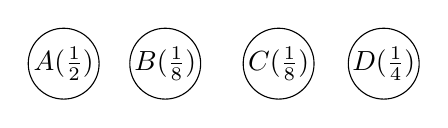
\begin{tikzpicture}[scale=0.15]
		      		\tikzstyle{every node}+=[inner sep=0pt]
		      		\draw [black] (26,-29.1) circle (3);
		      		\draw (26,-29.1) node {$A(\frac{1}{2})$};
		      		\draw [black] (34.6,-29.1) circle (3);
		      		\draw (34.6,-29.1) node {$B(\frac{1}{8})$};
		      		\draw [black] (44.2,-29.1) circle (3);
		      		\draw (44.2,-29.1) node {$C(\frac{1}{8})$};
		      		\draw [black] (53.1,-29.1) circle (3);
		      		\draw (53.1,-29.1) node {$D(\frac{1}{4})$};
		      	\end{tikzpicture}
		      \end{center}
		      		      
		\item Rendo, due nodi di frequenza più bassa, figli di un nuovo nodo di frequenza uguale alla somma dei figli, che chiamerò $\alpha$.
		      \begin{center}
		      	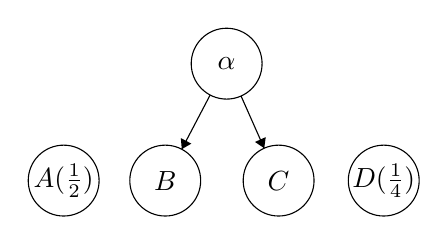
\begin{tikzpicture}[scale=0.15]
		      		\tikzstyle{every node}+=[inner sep=0pt]
		      		\draw [black] (26,-29.1) circle (3);
		      		\draw (26,-29.1) node {$A(\frac{1}{2})$};
		      		\draw [black] (34.6,-29.1) circle (3);
		      		\draw (34.6,-29.1) node {$B$};
		      		\draw [black] (44.2,-29.1) circle (3);
		      		\draw (44.2,-29.1) node {$C$};
		      		\draw [black] (53.1,-29.1) circle (3);
		      		\draw (53.1,-29.1) node {$D(\frac{1}{4})$};
		      		\draw [black] (39.8,-19.2) circle (3);
		      		\draw (39.8,-19.2) node {$\alpha$};
		      		\draw [black] (41.02,-21.94) -- (42.98,-26.36);
		      		\fill [black] (42.98,-26.36) -- (43.11,-25.42) -- (42.2,-25.83);
		      		\draw [black] (38.4,-21.86) -- (36,-26.44);
		      		\fill [black] (36,-26.44) -- (36.81,-25.97) -- (35.92,-25.5);
		      	\end{tikzpicture}
		      \end{center}
		      		      
		\item Continuo iterativamente, creo un nodo $\beta$ che ha per figli $\alpha$ e $D$.
		      \begin{center}
		      	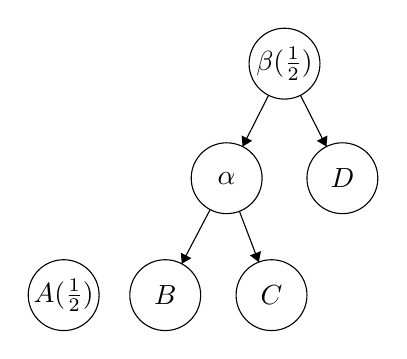
\begin{tikzpicture}[scale=0.15]
		      		\tikzstyle{every node}+=[inner sep=0pt]
		      		\draw [black] (26,-29.1) circle (3);
		      		\draw (26,-29.1) node {$A(\frac{1}{2})$};
		      		\draw [black] (34.6,-29.1) circle (3);
		      		\draw (34.6,-29.1) node {$B$};
		      		\draw [black] (43.6,-29.1) circle (3);
		      		\draw (43.6,-29.1) node {$C$};
		      		\draw [black] (49.6,-19.2) circle (3);
		      		\draw (49.6,-19.2) node {$D$};
		      		\draw [black] (39.8,-19.2) circle (3);
		      		\draw (39.8,-19.2) node {$\alpha$};
		      		\draw [black] (44.7,-9.5) circle (3);
		      		\draw (44.7,-9.5) node {$\beta(\frac{1}{2})$};
		      		\draw [black] (40.88,-22) -- (42.52,-26.3);
		      		\fill [black] (42.52,-26.3) -- (42.71,-25.37) -- (41.77,-25.73);
		      		\draw [black] (38.4,-21.86) -- (36,-26.44);
		      		\fill [black] (36,-26.44) -- (36.81,-25.97) -- (35.92,-25.5);
		      		\draw [black] (43.35,-12.18) -- (41.15,-16.52);
		      		\fill [black] (41.15,-16.52) -- (41.96,-16.03) -- (41.07,-15.58);
		      		\draw [black] (46.05,-12.18) -- (48.25,-16.52);
		      		\fill [black] (48.25,-16.52) -- (48.33,-15.58) -- (47.44,-16.03);
		      	\end{tikzpicture}
		      \end{center}
		      		      
		\item Un'ultima volta.
		      \begin{center}
		      	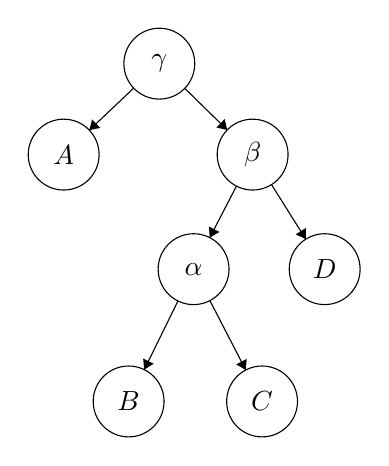
\begin{tikzpicture}[scale=0.15]
		      		\tikzstyle{every node}+=[inner sep=0pt]
		      		\draw [black] (28.8,-11.1) circle (3);
		      		\draw (28.8,-11.1) node {$A$};
		      		\draw [black] (34.3,-32) circle (3);
		      		\draw (34.3,-32) node {$B$};
		      		\draw [black] (45.6,-32) circle (3);
		      		\draw (45.6,-32) node {$C$};
		      		\draw [black] (50.9,-20.8) circle (3);
		      		\draw (50.9,-20.8) node {$D$};
		      		\draw [black] (39.8,-20.8) circle (3);
		      		\draw (39.8,-20.8) node {$\alpha$};
		      		\draw [black] (44.8,-11.1) circle (3);
		      		\draw (44.8,-11.1) node {$\beta$};
		      		\draw [black] (36.9,-3.4) circle (3);
		      		\draw (36.9,-3.4) node {$\gamma$};
		      		\draw [black] (41.18,-23.46) -- (44.22,-29.34);
		      		\fill [black] (44.22,-29.34) -- (44.3,-28.4) -- (43.41,-28.86);
		      		\draw [black] (38.48,-23.49) -- (35.62,-29.31);
		      		\fill [black] (35.62,-29.31) -- (36.42,-28.81) -- (35.53,-28.37);
		      		\draw [black] (43.43,-13.77) -- (41.17,-18.13);
		      		\fill [black] (41.17,-18.13) -- (41.99,-17.65) -- (41.1,-17.19);
		      		\draw [black] (46.4,-13.64) -- (49.3,-18.26);
		      		\fill [black] (49.3,-18.26) -- (49.3,-17.32) -- (48.45,-17.85);
		      		\draw [black] (34.73,-5.47) -- (30.97,-9.03);
		      		\fill [black] (30.97,-9.03) -- (31.9,-8.84) -- (31.21,-8.12);
		      		\draw [black] (39.05,-5.49) -- (42.65,-9.01);
		      		\fill [black] (42.65,-9.01) -- (42.43,-8.09) -- (41.73,-8.81);
		      	\end{tikzpicture}
		      \end{center}
		      		      
		\item Ecco il nostro albero di Huffman, completo di archi 0 e 1! I codici delle foglie andranno letti dal basso verso l'alto.
		      \begin{center}
		      	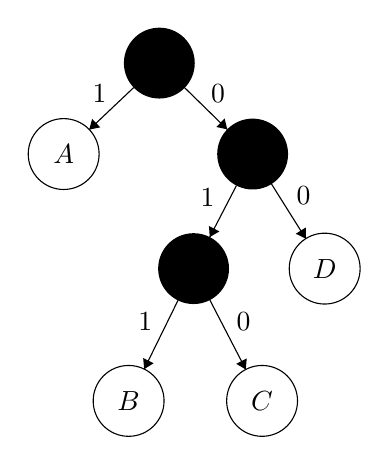
\begin{tikzpicture}[scale=0.15]
		      		\tikzstyle{every node}+=[inner sep=0pt]
		      		\draw [black] (28.8,-11.1) circle (3);
		      		\draw (28.8,-11.1) node {$A$};
		      		\draw [black] (34.3,-32) circle (3);
		      		\draw (34.3,-32) node {$B$};
		      		\draw [black] (45.6,-32) circle (3);
		      		\draw (45.6,-32) node {$C$};
		      		\draw [black] (50.9,-20.8) circle (3);
		      		\draw (50.9,-20.8) node {$D$};
		      		\fill [black] (39.8,-20.8) circle (3);
		      		\fill [black] (44.8,-11.1) circle (3);
		      		\fill [black] (36.9,-3.4) circle (3);
		      		\draw [black] (41.18,-23.46) -- (44.22,-29.34);
		      		\fill [black] (44.22,-29.34) -- (44.3,-28.4) -- (43.41,-28.86);
		      		\draw (43.39,-25.26) node [right] {$0$};
		      		\draw [black] (38.48,-23.49) -- (35.62,-29.31);
		      		\fill [black] (35.62,-29.31) -- (36.42,-28.81) -- (35.53,-28.37);
		      		\draw (36.35,-25.31) node [left] {$1$};
		      		\draw [black] (43.43,-13.77) -- (41.17,-18.13);
		      		\fill [black] (41.17,-18.13) -- (41.99,-17.65) -- (41.1,-17.19);
		      		\draw (41.61,-14.81) node [left] {$1$};
		      		\draw [black] (46.4,-13.64) -- (49.3,-18.26);
		      		\fill [black] (49.3,-18.26) -- (49.3,-17.32) -- (48.45,-17.85);
		      		\draw (48.48,-14.65) node [right] {$0$};
		      		\draw [black] (34.73,-5.47) -- (30.97,-9.03);
		      		\fill [black] (30.97,-9.03) -- (31.9,-8.84) -- (31.21,-8.12);
		      		\draw (31.83,-6.77) node [above] {$1$};
		      		\draw [black] (39.05,-5.49) -- (42.65,-9.01);
		      		\fill [black] (42.65,-9.01) -- (42.43,-8.09) -- (41.73,-8.81);
		      		\draw (41.87,-6.77) node [above] {$0$};
		      	\end{tikzpicture}
		      \end{center}
		      $$
		      A: 1; \ \ B : 011; \ \ C : 010; \ \ D : 00
		      $$
	\end{enumerate}
	\subsubsection{Implicazioni della codifica di Huffman}
	Per decodificare il file, bisogna avere una struttura dati contenente, appunto, la associazione stringa-simbolo della decodifica scelta.
	\subsection{Altri algoritmi di compressione lossless}
	\begin{itemize}
		\item \textbf{Run-Length-Encoding.}\\
		      Si basa sul comprimere una sequenza di bit (0 e 1) esprimendola in termini di numeri che indicano il numero di volte in cui si presenta 1, poi 0, poi 1, poi 0, poi $\dots$. Non è una codifica sempre vantaggiosa, ma nel caso in cui le sequenze di caratteri uguali sono molto lunghe, è il miglior modo per procedere. Agendo direttamente su i bit-planes, è un buon algoritmo.
		      		      
		\item \textbf{Codifica "differenziale".}\\
		      Per memorizzare una successione di valori, ad esempio numerici, \\potremmo memorizzare tutti i singoli elementi di questa successione. In alternativa, con la codifica differenziale, possiamo memorizzare il primo termine, poi la differenza tra il primo e il secondo, poi il secondo e il terzo, e così via.
		      $$
		      134,137,135,128, \dots \rightarrow(134) -3,+2,-7, \dots
		      $$
		      Come nella buona parte dei casi, usare questa codifica in combinazione con Huffman ci da ottimi risultati. La sequenza della codifica differenziale di una sequenza di numeri ha entropia più bassa dell'originale, aumentando l'efficacia di Huffman.\\
		      In generale, è sempre meglio si presentino elementi ridondanti per applicare compressioni di questo tipo.
	\end{itemize}
		
	\newpage 
		
	\section{La compressione lossy}
	La compressione lossy, come abbiamo già detto, implica la perdita di informazioni all'interno dei dati da comprimere. Tuttavia, l'informazione scelta per l'eliminazione, se fatta con buon criterio, ci permette di ottenere dati percepiti in maniera pressocché identica alla loro controparte originale. Eliminare alcuni bit-plane meno significativi nelle immagini, rimuovere nell'audio estremi di banda negli audio.\\
	Il PSNR ci offrirà informazioni utili legati alla qualità di un algoritmo di compressione lossy.\\
	In questo capitolo introdurremo adesso due algoritmi specifici per le immagini.
	\subsection{Requantization}
	Si tratta di una riduzione del numero di livelli di colore disponibili. In questo modo, andremo a risparmiare numero di bit dedicati a ciascun canale (RGB). Tuttavia, non sempre riquantizzare offre ottimi risultati.
		
	\newpage
		
	\section{JPEG}
	\subsection{Introduzione al JPEG}
	È l'acronimo di "Joint Photographic Experts Group", ed è dal 1992 ad oggi attualmente considerato uno standard ISO (per quanto in teoria non lo sia). È basato sulla DCT (Discrete Cosine Transform).\\
	È attualmente uno dei formati più importanti e usati di sempre. 
	\subsection{Passi fondamentali della codifica JPEG}
	\begin{enumerate}
		\item Pre-processing:
		      \begin{enumerate}
		      	\item Color Transform $(RGB \rightarrow YC_bC_r)$
		      	\item Sottocampionamento della crominanza
		      	\item Suddivisione della immagine in sottoimmagini
		      \end{enumerate}
		\item Trasformazione:
		      \begin{enumerate}
		      	\item Discrete Cosine Transform
		      	\item Quantization
		      \end{enumerate}
		      		      
		\item Codifica:
		      \begin{enumerate}
		      	\item DC ($(0,0)$) Coefficient Encoding
		      	\item Zig-zag ordering of AC Coefficients
		      	\item Entropy Coding (Huffman)
		      \end{enumerate}
	\end{enumerate}
		
	\newpage
		
	\section{Jpeg step-by-step}
	\subsection{Pre-Processing}
	\subsubsection{Passare a YCbCr}
	Il primo passaggio è una semplice conversione allo spazio di colore $YC_bC_r$, per separare le informazioni di luminanza rispetto a quelle di crominanza
	$$
	\begin{bmatrix}
		Y   \\
		C_b \\
		C_r 
	\end{bmatrix}
	=
	\begin{bmatrix}
		0.299 & 0.587  & 0.114  \\
		0.596 & -0.275 & -0.321 \\
		0.212 & -0.523 & 0.311  
	\end{bmatrix}
	\begin{bmatrix}
		R \\
		G \\
		B 
	\end{bmatrix}
	$$
	\subsubsection{Sottocampionamento della crominanza}
	I canali della crominanza sono meno importanti di quelli della luminanza, quindi, in questo step, si andrà a sottocampionare le informazioni relative ai canali $C_b$ e $C_r$, dimezzandone le dimensioni.
	In questo modo, a ogni 4 pixel di $Y$ corrisponde un pixel in $C_b$ e $C_r$.\\
	Questo è il primo passaggio lossy (e irreversibile) dell'algoritmo!
		
	\subsubsection{Suddivisione in sottoimmagini}
	Le immagini vengono suddivise in blocchi $8\times 8$.\\
	In questo modo verranno ottenute sotto-immagini dall'entropia minore e su cui sarà più semplice lavorare (considerandone anche le dimensioni).\\
	Ognuno di questi quadrotti $8\times 8$ sarà processati in maniera differente, ed è questo il motivo dietro al tipico artefatto a quadretti del JPEG.\\
	La quadrettatura è proporzionale alla compressione.
		
	\subsection{Trasformazione}
	\subsubsection{Passaggio preliminare - Shift dei livelli di grigio}
	Prima dell'applicazione della DCT, a ciascun pixel di ogni blocco viene sottratto un quantitativo pari a $2^{n-1}$, dove $n$ è il numero di bit dedicato a ciascun canale ($YC_bC_r$).\\
	In questo modo, il valore medio di grigio 128 diventerà 0, facilitando così alcuni prossimi passaggi.
		
	\newpage
		
	\subsubsection{DCT}
	Applichiamo la trasformata discreta del coseno ai 64 pixel dell'immagine.\\
	All'interno dei blocchi $8\times 8$, prima della DCT, i valori presenteranno correlazioni tra loro: la trasformata del coseno permetterà di ottenere valori non correlati tra loro (dimostrato statisticamente!), ottenendo dati a memoria zero\footnote{Stringhe a memoria zero, sono costituite da simboli indipendenti tra loro.
	In stringhe non a memoria zero, esiste una dipendenza tra i simboli che implica che la probabilità che un simbolo si presenti nella stringa, aumenta o diminuisce in funzione di altri simboli.}.
	$$
	F(u,v) = \frac{2}{N}\left[\sum^{N-1}_{x=0}\sum^{N-1}_{y=0}C(u)C(v)f(x,y)\cos\frac{(2x+1)u\pi}{2\cdot N}\cos\frac{(2y+1)v\pi}{2\cdot N} \right]
	$$
	$$
	f(x,y) = \frac{2}{N}\left[\sum^{N-1}_{u=0}\sum^{N-1}_{v=0}C(u)C(v)F(u,v)\cos\frac{(2x+1)u\pi}{2\cdot N}\cos\frac{(2y+1)v\pi}{2\cdot N} \right]
	$$
	In cui:
	$$
	C(u) = \frac{1}{\sqrt{2}} \text{ per } u=0; \ C(u) = 1 \text{ altrimenti}
	$$
	$$
	C(v) = \frac{1}{\sqrt{2}} \text{ per } v=0; \ C(v) = 1 \text{ altrimenti}
	$$
	In un blocco $8 \times 8$, a ogni coefficiente della matrice corrisponderà una base differente.
	Applicata la DCT, ci sarà possibile individure il coefficiente DC, ovvero l'elemento di coordinate $(0,0)$. Gli altri coefficienti saranno detti AC.\\
	Ricordiamo che tramite la DCT, ci sposteremo sul dominio delle frequenze. Le basi ottenute con la DCT coincidono a varie combinazioni di frequenze lungo le due dimensioni.
	\begin{figure}[htp]
		\centering
		\includegraphics[width=0.5\linewidth]{dct.png}
		\caption{Le basi ottenute con la DCT}
	\end{figure}
		
	\subsubsection{Quantizzazione}
	$$
	F_{quantizzato}= round(F/Q)
	$$
	La quantizzazione è irreversibile, e avviene arrotondando i valori della divisione tra i valori di $F$ e quelli di $Q$. La $Q$ è detta matrice di quantizzazione, e sarà differente tra il canale $Y$ e i canali $C_b,C_r$.\\
	La perdita delle informazioni è causata dall'arrotondamento, che rende irreversibile ottenere valori che divisi per $Q$ ritornano valori non interi.\\
	La matrice $Q$ dipende da un quality factor $QF$ che va da 1 a 100, e dalle matrici adottate da i produttori dei software / dispositivi di processing / ricezione dell'immagine.\\
	Il quality factor è inversamente proporzionale alla quantizzazione.
		
	\subsection{Codifica}
		
	\subsubsection{Zig-Zag ordering}
	Per applicare una codifica run-length, e preservare la coerenza tra i coefficienti vicini, andremo a linearizzare ogni blocco $8\times 8$ con un ordinamento a zig-zag.\\ Questo ordinamento a serpentina favorisce la creazione di lunghe sequenze continue di zeri.
		
	\subsubsection{Codifica coefficienti DC}
	I coefficienti DC, vengono codificati con una codifica differenziale, in quanto, presumibilmente, a DC di blocchi adiacenti saranno associati valori abbastanza simili.
		
	\subsubsection{Codifica coefficienti AC}
	I coefficienti AC, a differenza di quelli DC, vengono codificati all'interno del proprio blocco, ogni blocco indipendente dagli altri. Si è notato che, linearizzando i blocchi $8\times8$ a zig-zag, si ottiene una sequenza di valori che presentano con numerose sotto-sequenze di zeri.\\
	Si è deciso quindi di usare una codifica run-length skip value, in cui ogni valore viene codificato nel sequente modo:
	$$
	( \text{numero di 0 subito precedenti al numero } n \neq 0; n\neq 0)
	$$
		
	\newpage
	\subsubsection{Huffman}
	Viene usata successivamente una codifica di Huffman sulle differenze della codifica differenziale su DC e sui valori dei coefficienti AC.
		
	\subsubsection{Huffman sui DC}
	Sui valori continui DC, le differenze sono raggruppate in categorie. Indichieremo con $\Delta$ la differenza e con $SSSS$ la categoria. 
	A ogni codice $SSSS$ è associato un codice base. Una volta fatto ciò
	\begin{itemize}
		\item Con $\Delta>0$, i bit da aggiungere sono gli $n$ bit meno significativi del valore $\Delta$ in binario
		\item Con $\Delta<0$, i bit da aggiungere sono gli $n$ bit meno significativi del valore $\Delta$ in binario con complemento a due\footnote{Per rappresentare l'opposto di un numero binario in complemento se ne invertono, o negano, i singoli bit: si applica cioè l'operazione logica NOT. Si aggiunge infine 1 al valore del numero trovato con questa operazione. Tuttavia, in questo contesto, questo valore verrà successivamente rimosso.}, ai quali occorre sottrarre il valore 1.
		\item Con $\Delta=0$ siamo in un caso banale e la codifica rimane quella della tabella in $SSSS=0$, ovvero 010.
		      		          
	\end{itemize}
	N.B., le cifre sono aggiunte a destra rispetto al codice base.
		
	\subsubsection{Huffman sugli AC}
	Viene utilizzato un metodo simile.\\
	Una tabella associa ai valori dei coefficienti AC una categoria $SSSS$ che dipende dal valore $v$ della coppia $(0,v)$. Nella codifica run-length gli eventi sono espressi come coppie (run, categoria), dove run è la lunghezza della sequenza di zeri, e categoria è il valore di $SSSS$ del valore.
	\begin{itemize}
		\item Se $v>0$ i bit da aggiungere sono i bit meno significativi del valore $v$ in binario
		      		      
		\item Se $v<0$ i bit da aggiungere sono i bit meno significativi del valore in binario di $v$ con complemento a due ai quali occorre sottrarre il valore 1.
	\end{itemize}
	Inoltre, la tabella che associa (run,category) ai codici base, contiene anche la coppia $(0,0)$, alla quale associa il codice $1010 = EOB$, ovvero End of Block, fine del blocco. Indica la presenza del numero zero fino alla fine del blocco contenente i valori AC.
	\section{La ricostruzione delle immagini}
	Si deve tornare indietro ricostruendo i dati originali (o le loro approssimazioni per i passi irreversibili).\\
	Esistono varie strategie di ricostruzione dell'immagine, ma non le tratteremo nel corso.
		
	\subsection{JPEG: Input e Output a confronto}
	I blocchi ottenuti saranno differenti tra input e output. La differenza è inversamente proporzionale al quality factor.
		
	\subsection{JPEG su immagini grafiche}
	Dove sono presenti salti di colore importanti, come all'interno di immagini grafiche, JPEG tende a creare artefatti e colori non presenti molto evidenti all'interno delle immagini.\\
	Inoltre, JPEG non supporta il canale alfa, ovvero quello della trasparenza.
		
	\section{JPEG 2000}
	Sostituisce la DCT con le wavelets.\\
	Alloca più bit nelle zone con più informazioni e permette il controllo esplicito di tale allocazione.\\
	Raggiunge rapporti di compressione maggiori e non causa blocchettatura.\\
	Il formato JPEG 2000 non si è mai diffuso per inerzia tecnologica.
\end{document}